\documentclass[final, 12pt]{colt2018}

\usepackage{times}
%\usepackage[utf8]{inputenc} % allow utf-8 input
%\usepackage[T1]{fontenc}    % use 8-bit T1 fonts
%\usepackage{hyperref}       % hyperlinks
%\usepackage{url}            % simple URL typesetting
\usepackage{booktabs}       % professional-quality tables
\usepackage{amsfonts}       % blackboard math symbols
\usepackage{nicefrac}       % compact symbols for 1/2, etc.
%\usepackage{microtype}      % microtypography
\usepackage{enumitem}
%\usepackage{capt-of}
%\usepackage{lmodern}

\usepackage{amsmath,amssymb,mathrsfs}
%\usepackage[ruled, vlined, linesnumbered]{algorithm2e}
\PassOptionsToPackage{ruled, vlined, linesnumbered}{algorithm2e}
\usepackage{algorithm}
\usepackage[noend]{algpseudocode}
%\usepackage{algorithm2e}
%\usepackage{algorithmic}
%\usepackage{subfigure} % for using subfigure
%\usepackage{amsthm}
\newcommand{\exptext}[1]{\textcolor{red}{#1}}

\usepackage{graphicx}
\usepackage{mathtools}
\usepackage{footnote}
\usepackage{float}
\usepackage{xspace}
\usepackage{multirow}
%\usepackage{authblk}
\usepackage{wrapfig}
\usepackage{framed}

\usepackage{footnote}
\makesavenoteenv{tabular}
\makesavenoteenv{table}

%\usepackage[]{color-edits}
%\addauthor{HL}{blue}
%\addauthor{AA}{red}

\newcommand{\TVD}[1]{\norm{#1}_\text{TV}}

\newcommand{\EG}{\textsc{Epoch-Greedy}\xspace}
\newcommand{\EPG}{\textsc{$\epsilon$-Greedy}\xspace}
\newcommand{\minimonster}{\textsc{ILOVETOCONBANDITS}\xspace}
\newcommand{\ILTCB}{\textsc{ILTCB}\xspace}
\newcommand{\AdaEG}{\textsc{Ada-Greedy}\xspace}
\newcommand{\AdaILTCB}{\textsc{Ada-ILTCB}\xspace}
\newcommand{\AdaPE}{\textsc{Ada-PE}\xspace}
\newcommand{\AdaBIN}{\textsc{Ada-BinGreedy}\xspace}
\newcommand{\corral}{\textsc{Corral}\xspace}
\newcommand{\bistro}{\textsc{BISTRO+}\xspace}
\newcommand{\base}[1]{{{\cal{B}}_{#1}}}
\newcommand{\scale}{\rho}
\newcommand{\test}{\textsc{NonstatTest}\xspace}
\newcommand{\true}{\textit{True}\xspace}
\newcommand{\false}{\textit{False}\xspace}
\newcommand{\flag}{\textsc{flag}\xspace}
\newcommand{\bmu}{\bar{\mu}}

\newcommand{\calA}{{\mathcal{A}}}
\newcommand{\calB}{{\mathcal{B}}}
\newcommand{\calX}{{\mathcal{X}}}
\newcommand{\calS}{{\mathcal{S}}}
\newcommand{\calI}{{\mathcal{I}}}
\newcommand{\calJ}{{\mathcal{J}}}
\newcommand{\calK}{{\mathcal{K}}}
\newcommand{\calD}{{\mathcal{D}}}
\newcommand{\calE}{{\mathcal{E}}}
\newcommand{\calR}{{\mathcal{R}}}
\newcommand{\calT}{{\mathcal{T}}}
\newcommand{\calP}{{\mathcal{P}}}
\newcommand{\calQ}{{\mathcal{Q}}}
\newcommand{\calZ}{{\mathcal{Z}}}
\newcommand{\calM}{{\mathcal{M}}}
\newcommand{\avgR}{\wh{\cal{R}}}
\newcommand{\ips}{\wh{r}}
\newcommand{\whpi}{\wh{\pi}}
\newcommand{\whE}{\wh{\E}}
\newcommand{\whV}{\wh{V}}
\newcommand{\Reg}{\text{\rm Reg}}
\newcommand{\whReg}{\wh{\text{\rm Reg}}}
\newcommand{\flg}{\text{\rm flag}}
\newcommand{\one}{\boldsymbol{1}}
\newcommand{\var}{\Delta}
\newcommand{\bvar}{\bar{\Delta}}
\newcommand{\p}{\prime}
\newcommand{\evt}{\textsc{Event}}

\DeclareMathOperator*{\argmin}{argmin}
\DeclareMathOperator*{\argmax}{argmax}
\DeclareMathOperator*{\arginf}{arginf}
\DeclareMathOperator*{\argsup}{argsup}
\DeclareMathOperator*{\range}{range}
\DeclareMathOperator*{\mydet}{det_{+}}
\DeclarePairedDelimiter\abs{\lvert}{\rvert}
\DeclarePairedDelimiter\bigabs{\big\lvert}{\big\rvert}
\DeclarePairedDelimiter\ceil{\lceil}{\rceil}
\DeclarePairedDelimiter\floor{\lfloor}{\rfloor}
\DeclarePairedDelimiter\bigceil{\big\lceil}{\big\rceil}
\DeclarePairedDelimiter\bigfloor{\big\lfloor}{\big\rfloor}

\newcommand{\field}[1]{\mathbb{#1}}
\newcommand{\fY}{\field{Y}}
\newcommand{\fX}{\field{X}}
\newcommand{\fH}{\field{H}}
\newcommand{\fR}{\field{R}}
\newcommand{\fN}{\field{N}}
\newcommand{\E}{\field{E}}

\newcommand{\theset}[2]{ \left\{ {#1} \,:\, {#2} \right\} }
\newcommand{\inner}[1]{ \left\langle {#1} \right\rangle }
\newcommand{\Ind}[1]{ \field{I}_{\{{#1}\}} }
\newcommand{\eye}[1]{ \boldsymbol{I}_{#1} }
\newcommand{\norm}[1]{\left\|{#1}\right\|}
%\newcommand{\trace}[1]{\text{tr}\left({#1}\right)}
\newcommand{\trace}[1]{\textsc{tr}({#1})}
\newcommand{\diag}[1]{\mathrm{diag}\!\left\{{#1}\right\}}

\newcommand{\defeq}{\stackrel{\rm def}{=}}
\newcommand{\sgn}{\mbox{\sc sgn}}
\newcommand{\scI}{\mathcal{I}}
\newcommand{\scO}{\mathcal{O}}
\newcommand{\scN}{\mathcal{N}}

\newcommand{\dt}{\displaystyle}
\renewcommand{\ss}{\subseteq}
\newcommand{\wh}{\widehat}
\newcommand{\wt}{\widetilde}
\newcommand{\ve}{\varepsilon}
\newcommand{\hlambda}{\wh{\lambda}}
\newcommand{\yhat}{\wh{y}}

\newcommand{\hDelta}{\wh{\Delta}}
\newcommand{\hdelta}{\wh{\delta}}
\newcommand{\spin}{\{-1,+1\}}

%\newcommand{\theHalgorithm}{\arabic{algorithm}}

%\newtheorem{lemma}{Lemma}
%\newtheorem{theorem}{Theorem}
\newtheorem{cor}{Corollary}
%\newtheorem{remark}{Remark}
\newtheorem{prop}{Proposition}
%\newtheorem{definition}{Definition}
\newtheorem{assumption}{Assumption}

\newcommand{\paren}[1]{\left({#1}\right)}
\newcommand{\brackets}[1]{\left[{#1}\right]}
\newcommand{\braces}[1]{\left\{{#1}\right\}}

\newcommand{\normt}[1]{\norm{#1}_{t}}
\newcommand{\dualnormt}[1]{\norm{#1}_{t,*}}

\newcommand{\order}{\ensuremath{\mathcal{O}}}
\newcommand{\otil}{\ensuremath{\widetilde{\mathcal{O}}}}

\newcommand{\specialcell}[2][c]{\begin{tabular}[#1]{@{}c@{}}#2\end{tabular}}

\title{Efficient Contextual Bandits in Non-stationary Worlds}

% The \author macro works with any number of authors. There are two
% commands used to separate the names and addresses of multiple
% authors: \And and \AND.
%
% Using \And between authors leaves it to LaTeX to determine where to
% break the lines. Using \AND forces a line break at that point. So,
% if LaTeX puts 3 of 4 authors names on the first line, and the last
% on the second line, try using \AND instead of \And before the third
% author name.
 \coltauthor{\Name{Haipeng Luo} \Email{haipengl@usc.edu}\\
 \addr University of Southern California
 \AND
 \Name{Chen-Yu Wei} \Email{chenyu.wei@usc.edu}\\
 \addr University of Southern California
 \AND
 \Name{Alekh Agarwal} \Email{alekha@microsoft.com} \\
 \addr Microsoft Research, NYC
 \AND 
\Name{John Langford}\Email{jcl@microsoft.com} \\
 \addr Microsoft Research, NYC
 }

%\author{
%   Haipeng Luo \\
%   University of Southern California \\
%   \nolinkurl{haipengl@usc.edu} \\
%   \And
%   Alekh Agarwal \\
%   Microsoft Research, NYC \\
%   \nolinkurl{alekha@microsoft.com} \\
%   \And
%   John Langford \\
%   Microsoft Research, NYC \\
%   \nolinkurl{jcl@microsoft.com} \\ 
%}

\begin{document}
\maketitle

We present preconditioned stochastic gradient descent (SGD) algorithms for the $\ell_1$ minimization problem $\min_{\xx}\|\AA \xx - \bb\|_1$ in the overdetermined case, where there are far more constraints than variables. Specifically, we have $\AA \in \R^{n \times d}$ for $n \gg d$. Commonly known as the Least Absolute Deviations problem, $\ell_1$ regression can be used to solve many important combinatorial problems, such as minimum cut and shortest path. SGD-based algorithms are appealing for their simplicity and practical efficiency.
% Our algorithms precondition the matrix $\AA$ and then solve the problem for the resulting matrix $\tilde{\AA}$ using gradient descent techniques.
Our primary insight is that careful preprocessing can yield preconditioned matrices $\tilde{\AA}$ with strong properties (besides good condition number and low-dimension) that allow for faster convergence of gradient descent. In particular, we precondition using Lewis weights to obtain an isotropic matrix with fewer rows and strong upper bounds on all row norms. We leverage these conditions to find a good initialization, which we use along with recent smoothing reductions and accelerated stochastic gradient descent algorithms to achieve $\epsilon$ relative error in $\Otil(nnz(\AA) + d^{2.5} \epsilon^{-2})$ time with high probability, where $nnz(\AA)$ is the number of non-zeros in $\AA$. This improves over the previous best result using gradient descent for $\ell_1$ regression. We also match the best known running times for interior point methods in several settings.

Finally, we also show that if our original matrix $\AA$ is approximately isotropic and the row norms are approximately equal, we can give an algorithm that avoids using fast matrix multiplication and obtains a running time of $\Otil(nnz(\AA) + s d^{1.5}\epsilon^{-2} + d^2\epsilon^{-2})$, where $s$ is the maximum number of non-zeros in a row of $\AA$. In this setting, we beat the best interior point methods for certain parameter regimes.


%We consider the $\ell_1$ minimization problem $\min_{\xx}||\AA \xx - \bb||_1$ in the overconstrained case, where there are far more constraints than variables. More specifically, we have $\AA \in \R^{n \times d}$ for $n \gg d$. By using Lewis Weights preconditioning on $\AA$ and a careful initialization, we show that a standard stochastic gradient descent algorithm achieves $\epsilon$ relative error in about $nnz(\AA) +  d^3\epsilon^{-2}$ time with high probability. If we leverage smoothing reductions in \cite{AllenZhuH16} and the accelerated stochastic gradient descent algorithms in \cite{AllenZhu17}, we can achieve a running time of about $nnz(\AA) + d^{2.5}\epsilon^{-2}$ with the same guarantees. Both of these running times improve over the previous results in \cite{YangCRM16} and the latter result is comparable to the best known running times for interior point methods \cite{LeeS15}.
%
%The key idea will be to use our preconditioning to restrict our consideration to matrices $\AA$ such that $\AA^T\AA = \II$ and every row norm of $\AA$ is upper bounded by $O(\sqrt{d/n})$. \cite{cohenpeng} show that sampling $\AA$ with Lewis weights takes about $nnz(\AA) +d^{\omega}$ time and approximately preserves the minimization problem. Moreover, we can assume $n\le O(d\epsilon^{-2}\log n)$ for the sampled matrix. We then prove that all leverage scores of the sampled matrix are approximately equal. Since rotations preserve leverage scores, we can then rotate our sampled matrix to ensure that our desired properties are met in about $d^{\omega}\epsilon^{-2}$ time.
%
%Finally, we also show that if our original matrix $\AA$ is such that $\AA^T\AA \approx \II$ and the row norms of $\AA$ are bounded, we can avoid using fast matrix multiplication and prove a running time of about $nnz(\AA) + s d^{1.5}\epsilon^{-2}$, where $s$ is the maximum number of non-zeros in a row of $\AA$.

%Consequently, we will be able to restrict our consideration to matrices $A$ such that $A^TA \approx I$, and all row norms are equal, which is to say $||A_{i,:}||_2 = \sqrt{\frac{d}{n}}$ for all $i$.
%
%With a careful choice of our initial $x$, we show that standard gradient descent and stochastic gradient descent algorithms under these further assumptions only require $O(\frac{d}{\epsilon^2})$ and $O(\frac{d^2}{\epsilon^2})$ iterations, respectively, to achieve $\epsilon$ relative error with respect to the minimum objective value. Accordingly, these methods each achieve respective total runtime of $O(\frac{md}{\epsilon^2})$ and $O(\frac{d^3}{\epsilon^2})$, along with an $O(m)$ preconditioning cost, improving over the previous results in \cite{MahoneySGD}.
%
%We further examine the consequences of our assumptions when combined with smoothing reductions in [cite] and accelerated gradient descent techniques in [cite,cite]. As a result we are able to further improve the running times to $O(\frac{md}{\epsilon})$ and $O(dn\log{1/\epsilon} + \frac{d^2\sqrt{n}}{\epsilon})$.
%
%Random sampling $d\epsilon^{-2}\log{d}$ rows of $A$ will only incur error $\epsilon$ and reduces the latter running time to $O(\frac{d^{2.5}\log{d}}{\epsilon^2})$, which is then comparable to interior point methods of [cite]

% !TeX root = main.tex
\section{Introduction}
\label{sec:intro}
Generative models are often trained in an unsupervised fashion, fitting a model $q$ to a set of observed data $x_P \subseteq X$ drawn iid from some true distribution $p$ on $x\in X$. Now, of course $p$ may not exactly belong to family $Q$ of probability distributions being fit, whether $Q$ consists of Gaussians mixture models, Markov models, or even neural networks of bounded size. We first discuss the limitations of generative modeling without feedback, and then discuss our model and results.

%\subsection{Limitations of Generative Modeling from Positive Examples Alone}
Consider fitting a generative model on a text corpus consisting partly of poetry written by four-year-olds and partly of mathematical publications from the {\em Annals of Mathematics}. Suppose that learning to generate a poem that looks like it was written by a child was easier than learning to generate a novel mathematical article with a correct, nontrivial statement. If the generative model pays a high price for generating unrealistic examples, then it may be better off learning to generate children's poetry than mathematical publications. However, without negative feedback, it may be difficult for a neural network or any other model to know that the mathematical articles it is generating are stylistically similar to the mathematical publications but do not contain valid proofs.\footnote{This is excluding clearly fake articles published without proper review in lower-tier venues \citep{LabbeL13}.} 

As a simpler example, the classic Markovian ``trigram model'' of natural language assigns each word a fixed probability conditioned only on the previous two words. Prior to recent advances in deep learning, for decades the trigram model and its variant were the workhorses of language modeling, assigning much greater likelihood to natural language corpora than numerous linguistically motivated grammars and other attempts \citep{Rosenfeld00}. However, text sampled from a trigram is typically nonsensical, e.g., the following text was randomly generated from a trigram model fit on a corpus of text from the Wall Street Journal \citep{JurafskyM09}:
\begin{quote}
They also point to ninety nine point six billion dollars from two hundred
four oh six three percent of the rates of interest stores as Mexico and
gram Brazil on market conditions. 
\end{quote}

In some applications, like text compression using a language model \citep{WittenNC87}, maximizing likelihood is equivalent to optimizing compression. However, in many  applications involving generation, such nonsense is costly and unacceptable. Now, of course it is possible to always generate valid data by returning random training examples, but this is simply overfitting and not learning. Alternatively, one could incorporate human-in-the-loop feedback such as through crowdsourcing, into the generative model to determine what is a valid, plausible sentence.

In some domains, validity could be determined automatically. Consider a Markovian model of a well-defined concept such as mathematical formulas that compile in \LaTeX{}. Now, consider a $n$-gram Markovian character model which the probability of each subsequent character is determined by the previous $n$ characters. For instance, the expression \$\{2+\{x-y\}\$ is invalid in \LaTeX{} due to mismatched braces. For this problem, a \LaTeX{} compiler may serve as a validity oracle. Various $n$-gram models can be fit which only generate valid formulas. To address mismatched braces, for example, one such model would ensure that it always closed braces within $n$ characters of opening, and had no nested braces. While an $n$-gram model will not perfectly model the true distribution over valid \LaTeX{} formulas, for certain generative purposes one may prefer an $n$-gram model that generates valid formulas over one that assigns greater likelihood to the training data but generates invalid formulas. 

Figure \ref{fig:rectangle} illustrates a simple case of learning a rectangle model for data which is not uniform over a rectangle. A maximum likelihood model would necessarily be the smallest rectangle containing all the data, but most examples generated from this distribution may be invalid. Instead a smaller rectangle, as illustrated in the figure, may be desired.

\begin{figure}[h]\label{fig:rectangle}
\centering
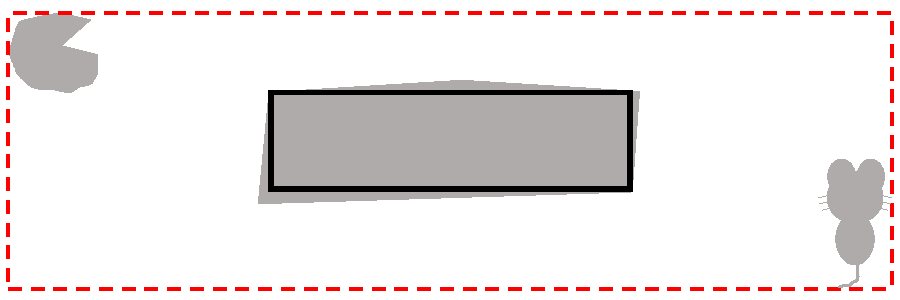
\includegraphics[width=3in]{fig.pdf}
\caption{Example where the underlying distribution $p$ is uniform over the (gray) valid regions. The solid rectangle maximizes our objective since it does not output nonsense (is supported only within the grey matter) and is closest to the $p$ (covers the maximum amount of grey matter). In contrast, the standard maximum likelihood (dashed red) rectangle must fully contain the observed samples, thus generating invalid points most of the time.  }
\end{figure}

Motivated by these observations, we evaluate a generative model $q$ on two axes. First is {\em coverage}, which is related to the probability assigned to future examples drawn from the true distribution $p$. Second is {\em validity}, defined as the probability that random examples generated from $q$ meet some validity requirement. Formally, we measure coverage in terms of a bounded {\em loss}:
$$\Loss(p,q)=\E_{x \sim p}[L(q_x)],$$
where $L:[0,1]\rightarrow [0,M]$ is a bounded decreasing function such as the capped log-loss $L(q_x)=\min(M, \log 1/q_x)$. % or $L(q_x)=\log 1/(q_x+\exp(-M))$. 
A bounded loss has the advantages of being efficiently estimable, and also it enables a model to assign 0 probability to one example (e.g., an outlier or error) if it greatly increases the likelihood of all other data. Validity is defined with respect to a set $V \subseteq X$, and $q(V)$ is the probability that a random example generated from $q$ lies within $V$. 

Clearly, there is a tradeoff between coverage and validity. We first focus on the case of (near) perfect validity. A Valid Generative Modeling (VGM) algorithm if it outputs, for a family of distributions $Q$ over $X$, if it outputs $\hat{q}$ with (nearly) perfect validity and whose loss is nearly as good as the loss of the best valid $q\in Q$. More precisely, $A$ is a VGM learner of $Q$ if for any nonempty valid subset $V \subseteq X$, any probability distribution $p$ over $V$, and any $\eps>0$, $A$ uses $n$ random samples from $p$ and makes $m$ membership oracle calls to $V$ and outputs a distribution $\hat{q}$ such that, $$\Loss(p, \hat{q}) \leq \min_{q \in Q: q(V)=1}\Loss(p,q) + \eps ~\text{ and }~\hat{q}(V)\geq 1-\eps.$$ 
We aim for our learner to be sample and query efficient, requiring that $n$ and $m$ are polynomial in $M, 1/\eps$ and a measure of complexity of our distribution class $Q$.
Furthermore, we would like our algorithms to be computationally efficient, with a runtime polynomial in the size of the data, namely the $n + m$ training examples. 
A more formal description of the problem is available in Section~\ref{sec:problem}.

$A$ is said to be {\em proper} if it always outputs $\hat{q}\in Q$ and {\em improper} otherwise.
In Section~\ref{sec:impossibility}, we first show that efficient proper learning for VGM is impossible. This is an information-theoretic result, meaning that even given infinite runtime and positive samples, one still cannot solve the VGM problem. Interestingly, this is different from binary classification, where it is possible to statistically learn from iid examples without a membership oracle.

Our first main positive result is an efficient (improper) learner for VGM. The algorithm relies on a subroutine that solves the following {\em Generative Modeling with Negatives} (GMN) problem: given sets $X_P, X_N \subset X$ of positive and negative examples, find the probability distribution $q \in Q$ which minimizes $\sum_{x \in X_P} L(q(x))$ subject to the constraint that $q(X_N)=0$. For simplicity, we present our algorithm for the case that the distribution family $Q$ is finite, giving sample and query complexity bounds that are logarithmic in terms of $|Q|$. However, as we show in Section~\ref{sec:infinite-families}, all of our results extend to infinite families $Q$. It follows that if one has a computationally efficient algorithm for the GMN problem for a distribution family $Q$, then our reduction gives a computationally efficient VGM learning algorithm for $Q$.

Our second positive result is an algorithm that minimizes $\Loss(p,q)$ subject to a relaxed validity constraint comparing against the optimal distribution that has validity $q(V)$ at least $1-\alpha$ for some $\alpha>0$. We show in Section~\ref{sec:partial-validity} that even in this more general setting, it is possible to obtain an algorithm that is statistically efficient but may not be computationally efficient. An important open question is whether there exists a computationally efficient algorithm for this problem when given access to an optimization oracle, as was the case for our algorithm for VGM.

\subsection{Related Work}
\cite{KearnsMRRSS94} showed how to learn distributions from positive examples in the realizable setting, i.e., where the true distribution is assumed to belong to the class being learned. In the same sense as their work is similar to PAC learning \citet{Valiant84} of distributions, our work is like agnostic learning \citet{KearnsSS94} in which no assumption on the true distribution is made. 

Generative Adversarial Networks (GANs)~\cite{GoodfellowPMXWOCB14} are an approach for generative modeling from positive examples alone, in which a generative model is trained against a discriminator that aims to distinguish real data from generated data. In some domains, GANs have been shown to outperform other methods at generating realistic-looking examples. Several shortcomings of GANs have been observed \citet{AroraRZ18}, and GANs are still subject to the theoretical limitations we argue are inherent to any model trained without a validity oracle. 

In supervised learning, there is a rich history of learning theory with various types of queries, including membership which are not unlike our (in)validity oracle. Under various assumptions, queries have been shown to facilitate the learning of complex classes such as finite automata \citet{Angluin88} and DNFs \citet{Jackson97}. See the survey of \cite{Angluin92} for further details.  Interestingly, \cite{Feldman09} has shown that for agnostic learning, i.e., without making assumptions on the generating distribution, the addition of membership queries does not enhance what is learnable beyond random examples alone. 
Supervised learning also has a large literature around active learning, showing how the ability to query examples reduces the sample complexity of many algorithms. See the survey of \cite{Hanneke14}. Note that the aim here is typically to save examples and not to expand what is learnable.
 
More sophisticated models, e.g., involving neural networks, can mitigate the invalidity problem as they often generate more realistic natural language and have even been demonstrated to generate \LaTeX{} that nearly compiles \citep{Karpathy15} or nearly valid Wikipedia markdown. However, longer strings generated are unlikely to be valid. For example, \cite{Karpathy15} shows generated markdown which includes:
\begin{quote}
==Access to ''rap===
The current history of the BGA has been [[Vatican Oriolean Diet]], British Armenian, published in 1893.  While actualistic such conditions such as the [[Style Mark Romanians]] are still nearly not the loss.
\end{quote}

Even ignoring the mismatched quotes and equal signs, note that this example has two so-called ``red links'' to two pages that do not exist. Without checking, it was not obvious to us whether or not Wikipedia had pages titled {\em Vatican Oriolean Diet} or {\em Style Mark Romanians}. In some applications, one may or may not want to disallow red links. In the case that they are considered valid, one may seek a full generative model of what might plausibly occur inside of brackets, as the neural network has learned in this case. If they are disallowed, a model might memorize links it has seen but not generate new ones. A validity oracle can help the learner identify what it should avoid generating.

 In practice, \cite{KusnerPH17} discuss how generative models from neural networks (in particular autoencoders) often generate invalid sequences. 
\cite{JanzWPKH18} learn the validity of examples output by a generative model using oracle feedback. 

%!TEX root = main.tex

\section{Preliminaries}
In this section, we will review some well-known results on~\gd~and~\nag~in the strongly convex setting, 
and existing results on convergence of~\gd~to second-order stationary points. 
% The pseudocode for these algorithms is given in Algorithms~\ref{algo:gd} and~\ref{algo:AGD} respectively.

% \cnote{Show gradient descent in equation}

\subsection{Notation}
Bold upper-case letters ($\A, \B$) denote matrices and bold lower-case letters ($\x, \y$) denote vectors. 
For vectors $\norm{\cdot}$ denotes the $\ell_2$-norm. For matrices, $\norm{\cdot}$ denotes the spectral norm and $\lambda_{\min}(\cdot)$ denotes the minimum eigenvalue.
For $f: \R^d \rightarrow \R$, $\grad f(\cdot)$ and  $\hess f(\cdot)$ denote its gradient and Hessian respectively, and $f^\star$ denotes its global minimum.
% Other than Section \ref{sec:related}, 
We use $O(\cdot), \Theta(\cdot), \Omega(\cdot)$ to hide absolute constants, and $\tilde{O}(\cdot), \tilde{\Theta}(\cdot), \tilde{\Omega}(\cdot)$ to hide absolute constants and polylog factors for all problem parameters. 
% \praneeth{I think it will be cleaner to make the dependence on smoothness parameters in Table~\ref{tab:main} and edit this statement} \jccomment{Then I also need to add function value dependence, maybe too complicated to compare}.\praneeth{The issue with this is that $O()$ is not just hiding constants but also problem dependent parameters. May be mention this explicitly in the caption to the table.} 
% We let $\ball^{(d)}_\x(r)$ denote the d-dimensional ball centered at $\x$ with radius $r$; when it is clear from context, we simply denote it as $\ball_\x(r)$. We use $\proj_{\mathcal{X}}(\cdot)$ to denote projection onto the set $\mathcal{X}$. Distance and projection are always defined in a Euclidean sense.


% \pn{Talk about ignoring $\log d$ factors in notation.}

\subsection{Convex Setting}\label{sec:prelim_convex}
% \begin{figure}[t]
% \begin{minipage}{0.5\textwidth}
% 	\begin{algorithm}[H]
% 	\caption{\gd($\x_0, \eta$)}\label{algo:gd}
% 	\begin{algorithmic}[1]
% 		\For{$t = 0, 1, \ldots, T $}
% 		\State $\x_{t+1} \leftarrow \x_t - \eta \grad f (\x_t)$
% 		\EndFor
% 		\State \textbf{return} $\x_T$
% 	\end{algorithmic}
% 	\end{algorithm}
% 	\vspace{0.5cm}
% \end{minipage}
% \begin{minipage}{.5\textwidth}

% \end{minipage}
% \end{figure}
To minimize a function $f(\cdot)$,~\gd ~performs the following sequence of steps:
\begin{equation*}
\x_{t+1} = \x_{t}- \eta \grad f(\x_t).
\end{equation*}
The suboptimality of~\gd~and the improvement achieved by~\nag~can be clearly illustrated for the case of smooth and strongly convex functions. %The definitions of smoothness and strong convexity are as follows.
\begin{definition}\label{def:smooth}
A differentiable function $f(\cdot)$ is \textbf{$\ell$-smooth (or $\ell$-gradient Lipschitz)} if:
\begin{equation*}
\norm{\grad f(\x_1) - \grad f(\x_2)} \le \ell \norm{\x_1 - \x_2} \quad \forall \; \x_1, \x_2.
\end{equation*}
\end{definition}
\noindent
The gradient Lipschitz property asserts that the gradient can not change too rapidly in a small local region.
\begin{definition}\label{def:convex}
A twice-differentiable function $f(\cdot)$ is \textbf{$\alpha$-strongly convex} if
$\lambda_{\min}(\hess f(\x)) \ge \alpha, \;  \forall \; \x$.
% $f(\x_2) \ge f(\x_1) + \la \grad f(\x_1), \x_2 - \x_1 \ra + \frac{\alpha}{2}\norm{\x_2 - \x_1}^2, \quad \forall \; \x_1, \x_2.$
\end{definition}
Let $\fstar \defeq \min_{\y}f(\y)$. A point $\x$ is said to be \textbf{$\epsilon$-suboptimal} if $f(\x)  \le  \fstar + \epsilon$. The following theorem gives the convergence rate of GD and AGD for smooth and strongly convex functions.
\begin{theorem}[\cite{nesterov2004introductory}]\label{thm:gd_convex}
Assume that the function $f(\cdot)$ is $\ell$-smooth and $\alpha$-strongly convex. Then, for any $\epsilon>0$,
the iteration complexities to find an $\epsilon$-suboptimal point are as follows:
\begin{itemize}
\item GD with $\eta  = 1/\ell$: \quad $O((\ell/\alpha) \cdot \log ((f(\x_0) - \fstar)/\epsilon))$
\item AGD (Algorithm~\ref{algo:AGD}) with $\eta = 1/\ell$ and $\theta = \sqrt{\alpha/\ell}$:
\quad$O(\sqrt{\ell/\alpha} \cdot \log ((f(\x_0) - \fstar)/\epsilon))$.
\end{itemize}
% ~\gd~with $\eta = \frac{1}{\ell}$ will output an \ESP ~in iterations:
% \begin{equation*}
% O\left(\frac{\ell}{\alpha}\log \frac{f(\x_0) - \fstar}{\epsilon}\right).
% \end{equation*}
\end{theorem}

The number of iterations of GD depends linearly on the ratio $\ell/\alpha$, which is called the condition number of $f(\cdot)$ since $\alpha \I \preceq\hess f(\x) \preceq \ell \I $. Clearly $\ell \geq \alpha$ and hence condition number is always at least one. Denoting the condition number by ${\cn}$, we highlight two important aspects of~\nag: (1) the momentum parameter satisfies $\theta = 1/\sqrt{\cn}$ and (2) \nag~improves upon GD by a factor of $\sqrt{\cn}$. 
% The following theorem gives the convergence rate of~\nag~for these problems.
% \begin{theorem}[\cite{nesterov2004introductory}]\label{thm:agd_convex}
% Assume that the function $f(\cdot)$ is $\ell$-smooth and convex. Then, for any $\epsilon>0$,~\nag~with $\eta = \frac{1}{\ell}$ and $\theta = \Theta(\sqrt{\frac{\alpha}{\ell}}) $ will output an~\ESP~in iterations:
% \begin{equation*}
% O\left(\sqrt{\frac{\ell}{\alpha}}\log \frac{f(\x_0)-\fstar }{\epsilon}\right).
% \end{equation*}
% \end{theorem}
% \noindent
% Note that the rate here improves upon that of~\gd~by a factor of $\sqrt{\frac{\ell}{\alpha}}$ i.e., squareroot of the condition number.
%say something about condition number.

\subsection{Nonconvex Setting}
For nonconvex functions finding global minima is NP-hard in the worst case. The best one can hope for in this setting is convergence to stationary points. There are various levels of stationarity.
\begin{definition}
$\x$ is an \textbf{\EFSP} of function $f(\cdot)$ if $\norm{\grad f(\x)} \le \epsilon$.
\end{definition}
\noindent
As mentioned in Section~\ref{sec:intro}, for most nonconvex problems encountered in practice, a majority of first-order stationary points turn out to be saddle points. Second-order stationary points require not only zero gradient, but also positive semidefinite Hessian, ruling out most saddle points.
%Therefore, this paper focus on finding second-order stationary point.
%In order to discuss Hessian-related properties meaningfully, we first need to assert Hessian smoothness condition.
Second-order stationary points are meaningful, however, only when the Hessian is continuous.
% second order stationary points which means that in addition to being first order stationary points, the Hessian at these points is almost positive semidefinite. This is meaningful only if the Hessian does not change arbitrarily (and perhaps have large negative eigenvalues) in a small neighborhood around this point. In other words, finding second order stationary points is meaningful only if the Hessian is continuous.
%\cnote{Should we talk the case where gradient is Lipschitz but Hessian is not?}
% \begin{theorem}[\citep{nesterov1998introductory}]\label{thm:grad_smooth}
% Assume that the function $f(\cdot)$ is $\ell$-smooth. Then, for any $\epsilon>0$, gradient descent will output an \EFSP ~in iterations:
% \begin{equation*}
% \frac{\ell(f(\x_0) - f^\star)}{\epsilon^2}.
% \end{equation*}
% \end{theorem}
\begin{definition}\label{def:HessianLip}
A twice-differentiable function $f(\cdot)$ is \textbf{$\rho$-Hessian Lipschitz} if:
\begin{equation*}
\norm{\hess f(\x_1) - \hess f(\x_2)} \le \rho \norm{\x_1 - \x_2} \quad \forall \; \x_1, \x_2.
\end{equation*}
\end{definition}
%\noindent
% For Hessian Lipschitz functions, we recall the definition of second order stationary points from~\cite{nesterov2006cubic}.
\begin{definition}[\cite{nesterov2006cubic}]\label{def:SOSP}
For a $\rho$-Hessian Lipschitz function $f(\cdot)$, $\x$ is an \textbf{\ESSP} if:
% $\norm{\grad f(\x)} \le \epsilon$ and $\lambda_{\min}(\hess f(\x)) \ge - \sqrt{\rho \epsilon}$.
\begin{equation*}
\norm{\grad f(\x)} \le \epsilon \quad\text{and}\quad \lambda_{\min}(\hess f(\x)) \ge - \sqrt{\rho \epsilon}.
\end{equation*}
\end{definition}
\noindent
The following theorem gives convergence rate of perturbed~\gd~to second-order stationary points.
%See~\cite{jin2017escape} for a detailed description of the algorithm.
\begin{theorem}[\citep{jin2017escape}]\label{thm:perturbed_GD}
Assume that the function $f(\cdot)$ is $\ell$-smooth and $\rho$-Hessian Lipschitz. Then, for any $\epsilon>0$, perturbed GD outputs an \ESSP ~w.h.p in iterations:
\begin{equation*}
\otilde{\frac{\ell(f(\x_0) - \fstar)}{\epsilon^2}}.
\end{equation*}
\end{theorem}
\noindent
Note that this rate is essentially the same as that of~\gd~for convergence to first-order stationary points. In particular, it only has polylogarithmic dependence on the dimension.

\section{Tolerant Testing for Unions of $d$ Intervals}
\label{sec:interval}
%In this section, we consider the concept class $\dintervals$ of binary functions $f$ defined on $\mathbb{R}$ such that $f^{-1}(1)$ is a union of at most $d$ intervals. We use $\udi_{\calD}(f,\epsilon,d)$ to denote the distance approximation task $\da_{\calD}(f,\epsilon)$ when the underlying hypothesis class is the class $\interval(d)$ of unions of $d$ intervals. We show (Theorem \ref{thm:main}) that there is an $\udi_{\calD}(f,\epsilon,d)$ algorithm in the active model with query complexity independent of $d$ even when the data distribution is unknown to the algorithm.

\begin{theorem}[main theorem]
\label{thm:main}
Suppose $\calC$ is the class of functions $f:\mathbb{R}\rightarrow \{0,1\}$ satisfying $f^{-1}(1)$ is a union of at most $d$ intervals for $d>0$. Given $\epsilon\in(0,\frac 12)$, there is a tolerant tester for $\calC$ in the active testing model with respect to an arbitrary unknown distribution $\calD$ on $\mathbb{R}$ with additive error $\epsilon$ using $O(\frac{1}{\epsilon^6}\log\frac{1}{\epsilon})$ queries on $O(\frac{d}{\epsilon^2}\log\frac{1}{\epsilon})$ unlabeled examples.
%Suppose $d>0$ and $\epsilon\in (0,\frac{1}{2})$ are given as input. Let $\mathcal{D}$ be a distribution over $\mathbb{R}$ unknown to the tester. Given \emph{active} access to an input function $f:\mathbb{R}\rightarrow \{0,1\}$ with respect to $\calD$, there is an $\udi_{\calD}(f\ac,\epsilon,d)$ tester using $O(\frac{1}{\epsilon^6}\log\frac{1}{\epsilon})$ queries on $O(\frac{d}{\epsilon^2}\log\frac{1}{\epsilon})$ unlabeled examples.
\end{theorem}

We summarize the proof of Theorem \ref{thm:main} as follows and present the full proof in Appendix \ref{sec:proofmain}.

Let's first consider the case when $\calD$ is the uniform distribution $\calU$ over $[0,1]$, and then extend to the arbitrary unknown distribution case. The tester first partitions $[0,1]$ into $m$ pieces, $X_1=[0,\frac{1}{m}],X_2=(\frac{1}{m},\frac{2}{m}],X_3=(\frac{2}{m},\frac{3}{m}],\cdots,X_m=(\frac{m-1}{m},1]$. $\forall 1\leq i\leq m,\forall k\in\mathbb{N}$, we define $\calC_i^k$ to be the class of binary functions $f$ on $X_i$ such that $f^{-1}(1)$ is a union of at most $k$ intervals. Note that $\calC_i^0\neq\emptyset$. Therefore, we can define $\property$, the composition of $m$ additive properties as in Section \ref{sec:composition}. 

Note that for any $d'>0$ and any truncation $t>0$, the concept class $\property^{t}(d')$ has VC-dimension at most $2d'$. Therefore, according to the VC Theory for agnostic learning, we have a $(d',l,t,\epsilon')$ distance approximation oracle using $O(\frac{d'}{{\epsilon'}^2}\log\frac{1}{\epsilon'})$ queries and unlabeled examples simply by empirical risk minimization. By the Composition Lemma (Lemma \ref{thm:additive}), the tester calls the oracle once for $d'=(1+\frac\mu 2)(1+\frac\epsilon 8)\lambda l,l=O(\frac 1{\epsilon'\mu}+\frac 1{{\epsilon'}^2}),t=\frac{4(1+\frac\epsilon 8)\lambda}{\epsilon'},\epsilon'=\frac{\epsilon}{4}$ and implements an $(\frac{\epsilon}{2},1+\mu)$-bi-criteria distance approximation algorithm for $\property((1+\frac{\epsilon}{8})\lambda m)=\property((1+\frac{\epsilon}{8})d)$. We claim that this algorithm is automatically a tolerant tester for the class of unions of $d$ intervals within additive error at most $\epsilon$ if we choose $1+\mu=\frac{1+\frac\epsilon 4}{1+\frac\epsilon 8}$. 

Note that the active tester for the uniform distribution over $[0,1]$ implies a query tester for the same distribution with the same query complexity. As pointed out by \citet{BBBY12}, the query tester for the uniform distribution over $[0,1]$ then implies a query tester for arbitrary (known) distribution with the same query complexity. According to Lemma \ref{thm:reductiontoquery}, the query tester for an arbitrarily given distribution can be finally transformed to an active tester for arbitrary (unknown) distribution with the same query complexity and unlabeled sample complexity $O(\frac{d}{\epsilon^2}\log\frac{1}{\epsilon})$.



\section{Implications}\label{sec:implications}
In this section we discuss the implications of interval regret
guarantees on switching/dynamic regret, both of which are
meaningful performance measures for non-stationary environments.

%\subsection{Switching Regret}\label{subsec:switching}
\paragraph{Switching Regret.} We begin with switching regret, which is pretty straightforward.
One only needs to divide the entire time interval $[1,T]$ into several i.i.d. subintervals with length bounded by $L$,
and then apply the interval regret guarantee on each of these subintervals since the best policy $\pi^\star_t$ remains the same on each of these subintervals
(for \AdaEG and \AdaILTCB we can simply set the variation tolerance $v$ to be $0$).
We take Exp4.S as an example and state the results below 
(see Appendix~\ref{app:Exp4.S} for the proof),
while similar results for other algorithms are summarized in Table~\ref{tab:results}.
%but one can easily generalize the results to the other algorithms we have presented
%with different conditions and regret rates (see Table~\ref{tab:results}).

\begin{cor}\label{cor:Exp4.S} 
Exp4.S with parameter $L$ ensures $\E\left[ \sum_{t=1}^T r_t(\pi_t^\star(x_t)) - r_t(a_t) \right] \leq 
\otil\left(\left(\frac{T}{\sqrt{L}} + S\sqrt{L}\right) \sqrt{K\ln N}\right)$ where $S = 1 + \sum_{t=2}^T \one\{\calD_t \neq \calD_{t-1}\}$.
\end{cor}


If $S$ is known, then setting $L = T/S$ gives a bound of $\otil(\sqrt{STK\ln N})$.
Otherwise setting $L$ with different values leads to different bounds that are incomparable.
For example, setting $L = T$ leads to $\otil(S\sqrt{TK\ln N})$ while setting 
$L = \sqrt{T}$ leads to $\otil((T^\frac{3}{4} + ST^\frac{1}{4})\sqrt{K\ln N})$.
No matter how $L$ is tuned, however,
these bounds all become vacuous ($\Omega(T)$) when $S$ is large enough but still sublinear in $T$,
an issue addressed later in Section~\ref{sec:bin}.

%\subsection{Dynamic Regret}\label{subsec:dynamic}
\paragraph{Dynamic Regret.}
%All results with efficient algorithms presented so far require some
%additional conditions to obtain meaningful bounds.  We now drop any of
%these assumptions and move on to bounding dynamic regret in terms of
We now move on to discuss dynamic regret in terms of the variation measures $\var$ or $\bvar$ (recall $\var = \sum_{t=2}^T \max_{\pi \in \Pi} |\calR_t(\pi) - \calR_{t-1}(\pi)|$ and $\bvar = \sum_{t=2}^T \TVD{\calD_t-\calD_{t-1}}$). %(recall their definitions in Section~\ref{sec:setup}).
We first point out that previous
works~\citep{BesbesGuZe15, ZhangYaJiZh17} have studied a reduction
from dynamic regret to interval regret, restated below:

\begin{lemma}\label{lem:dynamic2interval}
Let $\{\calI_i = [s_i, t_i]\}_{i \in [n]}$ be time intervals that partition $[1,T]$. 
We have 
\[
\sum_{t=1}^T \E_t\left[ r_t(\pi^\star_t(x_t)) - r_t(a_t) \right] \leq
\sum_{i=1}^n \sum_{t\in\calI_i} \E_t\left[ \left(
  r_t(\pi^\star_{s_i}(x_t)) - r_t(a_t) \right)\right] +
2\sum_{i\in[n]} |\calI_i|\var_{\calI_i}.
\]
\end{lemma}

We include the proof in Appendix~\ref{app:dynamic2interval} for
completeness.  Partitioning $[1,T]$ into intervals with equal length $L'
\leq L$, applying this lemma and Theorem~\ref{thm:Exp4.S},
and using the fact $\sum_{i\in[n]} \var_{\calI_i} \leq \var$ directly
lead to the following result for Exp4.S.

\begin{cor}\label{thm:Exp4.S_dynamic}
Exp4.S with parameter $L$ ensures that $\E\left[ \sum_{t=1}^T
  r_t(\pi^\star_t(x_t)) - r_t(a_t) \right] \leq \otil\left(\min_{0\leq
  L' \leq L} \left\{\frac{T}{L'}\sqrt{LK\ln N} + L'\var\right\} \right)$.
\end{cor}

Again, if $\var$ is known one can tune $L$
optimally to get a bound $\otil(T^\frac{2}{3}(\Delta K\ln
N)^\frac{1}{3} + \sqrt{TK\ln N})$, similar to the optimal
dynamic regret in multi-armed bandits~\citep{BesbesGuZe14}.  When
$\Delta$ is unknown, different values of $L$ give different and in
general incomparable bounds.  For example, setting $L =
T^\frac{2}{3}$ leads to $\otil(T^\frac{2}{3}\sqrt{\var}(K\ln
N)^\frac{1}{4} +T^\frac{2}{3}\sqrt{K\ln N})$
(with $L' = \min\{T^{2/3}, T^{2/3}(K\ln N)^{1/4}/\sqrt{\var}\}$ in this case),
which is again vacuous for large $\var$.

Similar arguments also provide a dynamic regret bound for \corral with \bistro in the transductive setting,
as shown in Table~\ref{tab:results} (also see Corollary~\ref{cor:BISTRO+_dynamic} in Appendix~\ref{app:BISTRO+}).
However, the exact same argument above does not apply to \AdaEG and \AdaILTCB
directly since its interval regret guarantee requires $\var_\calI \leq
v$.  
It turns out, however, one can set $v$ to some carefully selected value and
partition $[1,T]$ correspondingly so that every subinterval satisfies $|\calI| \leq L$
and $\var_\calI \leq v$,
to obtain the following results
that hold in a completely adversarial setting.\footnote{The dependence on
  $K\ln(N/\delta)$ in these results is slightly loose for conciseness and could be tightened.}
  The proofs are included in Appendix~\ref{app:dynamic2interval}.

\begin{cor}
\label{cor:dynamic AdaEG}
With probability at least $1 - \delta$, \AdaEG with parameter $L$, $\delta$ and
$v = L^{-1/3}$ ensures that
\[
\sum_{t=1}^T r_t(\pi_t^\star(x_t)) - r_t(a_t) \leq
\otil\left(\left(  \frac{T}{L^{1/3}} + L^{1/3}\sqrt{\var T}
\right)K\ln(N/\delta)\right).
\]
Specifically, if $\var$ is known, setting $L =
\min\{(T/\var)^\frac{3}{4}, T\}$ gives
$\otil((\var^\frac{1}{4}T^\frac{3}{4} +
T^\frac{2}{3})K\ln(N/\delta))$; otherwise, setting $L = T^\frac{3}{4}$
gives $\otil((\sqrt{\var}+1)T^\frac{3}{4} K\ln(N/\delta))$.
\end{cor}

%Again, with \AdaILTCB we obtain the following stronger result (in terms of $\bvar$) by the same argument.

\begin{cor}
\label{cor:dynamic AdaILTCB}
With probability at least $1 - \delta$, \AdaILTCB with parameter $L$, $\delta$ and
$v = L^{-\frac{1}{2}} $ ensures that
\[
\sum_{t=1}^T r_t(\pi_t^\star(x_t)) - r_t(a_t) \leq
\otil\left(\left(\frac{T}{\sqrt{L}} + \bvar L
\right)K\ln(N/\delta)\right).
\]
If $\bvar$ is known, setting $L =
\min\{(T/\bvar)^\frac{2}{3}, T\}$ gives
$\otil((\bvar^\frac{1}{3} T^\frac{2}{3} +\sqrt{T})K\ln(N/\delta))$; otherwise, setting $L = T^\frac{2}{3}$
gives $\otil((\bvar+1) T^\frac{2}{3} K\ln(N/\delta))$.
\end{cor}

One can see that again the result for \AdaILTCB is better than that of \AdaEG,
and is in fact very close to that of the inefficient baseline Exp4.S,
except that it is in terms of the slightly larger variation measure $\bvar$.

%%%%%%%%%%%%%%%%%%%%%%%%%%%%%%%%%%%
%        Commented out the original version
%%%%%%%%%%%%%%%%%%%%%%%%%%%%%%%%%%%
\iffalse
It turns out, however, one can simply set $v= B(L)$ and
partition $[1,T]$ in a more careful way to obtain the following result
that holds in a complete adversarial setting.

\begin{cor}
With probability at least $1 - \delta$, \AdaEG with parameter $L$, $\delta$ and
$v = B(L)$ ensures that
\footnote{For simplicity, in this bound the dependence on the term
  $K\ln(N\delta)$ is slightly loose and could be tightened.}
\[
\sum_{t=1}^T r_t(\pi_t^\star(x_t)) - r_t(a_t) \leq
\otil\left(\left(\frac{T}{L^\frac{1}{3}} + L\var_T
\right)K\ln(N/\delta)\right).
\]
Specifically, if $\var_T$ is known, setting $L =
\min\{(T/\var_T)^\frac{3}{4}, T\}$ gives
$\otil((T^\frac{3}{4}\var_T^\frac{1}{4} +
T^\frac{2}{3})K\ln(N/\delta))$; otherwise, setting $L = T^\frac{3}{4}$
gives $\otil(T^\frac{3}{4}(\var_T+1) K\ln(N/\delta))$.
\end{cor}

\begin{proof}
The proof of Theorem~\ref{thm:AdaEG2} shows that with probability at
least $1 - \delta/2$, \AdaEG ensures that for any interval $\calI$
such that $|\calI| \leq L$ and $\var_\calI \leq B(L)$, we have
$\sum_{t \in \calI} \E_t[ r_t(\pi^\star_t(x_t)) - r_t(a_t)] \leq
\otil\left(L^\frac{2}{3}\sqrt{K\ln(N/\delta)} +
K\ln(N/\delta)\right)$.  We can thus first partition $[1, T]$ evenly
into $T/L$ intervals, then within each interval, further partition it sequentially
into several largest subintervals so that for each of them the variation is at
most $B(L)$. Since the total variation is $\var_T$, it is clear that
this results in at most $T/L + \var_T/B(L)$ subintervals, each of
which satisfies the conditions of Theorem~\ref{thm:AdaEG2}. Applying
Lemma~\ref{lem:dynamic2interval} and Hoeffding-Azuma inequality then
lead to the claimed bound.
\end{proof}



\begin{cor}
With probability at least $1 - \delta$, \AdaILTCB with parameter $L$, $\delta$ and
$v = ?$ ensures that
\[
\sum_{t=1}^T r_t(\pi_t^\star(x_t)) - r_t(a_t) \leq
\otil\left(\right).
\]
\end{cor}

\fi
%It is not surprising that the dynamic regret of \AdaEG is again worse
%than the one of Exp4.S.  It is not clear though whether (variants) of
%\AdaILTCB could achieve similar results as Exp4.S.  It appears that
%not only the variation of $\calR_t(\pi)$, but also the variation of
%$\E_{x\sim \calD_t^\calX} [\frac{1}{Q(\pi(x)|x)}]$ matters in this
%case.  We leave this problem as a future direction.


\section{Achieving Switching/Dynamic Regret with No Parameters}
\label{sec:bin}

\begin{algorithm}[t]
\SetAlgoLined
\setcounter{AlgoLine}{0}
\SetAlgoVlined
\DontPrintSemicolon
\caption{\AdaBIN}\label{alg:AdaGreedy.bin}
\nl {\bf Input}: allowed failure probability $\delta$ \\ 
\nl {\bf Define}:
$\beta_\calI= 2\sqrt{\frac{\ln(4T^2N/\delta)}{\mu_\calI \abs{\calI}}}+\frac{\ln(4T^2N/\delta)}{\mu_\calI \abs{\calI}}$, where $\displaystyle\mu_\calI\triangleq \min_{t\in\calI} \mu_t$ and $\mu_t$ is defined below, $\alpha_\calI = 2\sqrt{\frac{K\ln(4T^2N/\delta)}{\abs{\calI}}}+\frac{K\ln(4T^2N/\delta)}{\abs{\calI}}$\\
\nl {\bf Initialize}: $t=1$, $i=1$, $T_1=0$ \Comment{$i$ indexes an epoch}\label{line:rerun_beginning2}\\
\nl\label{line:adagreedy restart}\For(\Comment{$j$ indexes a block}){$j=1, 2, \ldots$}{ 
\nl Compute $\hat{\pi}_{(i,j)} = \argmax_{\pi\in\Pi}\avgR_{[T_i+1, T_i+2^{j-1}-1]}(\pi)$ 
\Comment{or arbitrary if $j=1$}\\
\nl $H=2^{j-1}$ \Comment{$H$ is block length}\\
%\nl $\triangleright$ {Divide block $j$, which has length $H$, into bins of length $H^\gamma$ \footnotemark{\label{same}}} \\
\nl\label{line:forloop of bin}\For(\Comment{$b$ indexes a bin, each with length $\sqrt{H}$}){$b = 1, 2, \ldots, \sqrt{H}$}{
\nl\label{line:exploration prob}Make bin $b$ an exploration bin with probability $1/\sqrt{b}$; otherwise an exploitation bin\\
\nl\label{line:forloop of bin step}\For(\Comment{loop through rounds in bin $b$}){$\tau = 1, \ldots, \sqrt{H}$}{
\nl       Let $\mu_t=\min\Big\{ \frac{1}{K}, (t-T_i)^{-\frac{1}{3}}\sqrt{\frac{\ln(N/\delta)}{K}} \Big\}$\\
\nl       Set $p_t(a)=\begin{cases}
             \frac{1}{K}, &\text{if bin $b$ is an exploration bin}, \\
             \mu_t+(1-K\mu_t)\one \{ a=\hat{\pi}_{(i,j)}(x_t) \}, &\text{if bin $b$ is an exploitation bin}.
          \end{cases}$ \\
\nl       Play $a_t\sim p_t$ and receive $r_t(a_t)$ \\
%\nl       $\triangleright$ {Call \test only when $b$ is an exploration bin} \\
\nl\label{line:trigger_rerun_ada3}  \If{$j>1$ and (bin $b$ is exploration bin) and ($\test(t)=\true$)}{
\nl                  $T_{i+1}\leftarrow t$, $t\leftarrow t+1$, $i\leftarrow i+1$ \\ 
\nl                  \textbf{goto} Line~\ref{line:adagreedy restart}
              }
\nl           $t\leftarrow t+1$
          }
      }
      }
\ \\
\textbf{Procedure\ }$\test(t)$\\
\nl $\ell=1$ \\
\nl \While{$[t-\ell+1, t]$ is a subset of the current bin}{
\nl    Let $A\triangleq [t-\ell+1,t]$ and $B\triangleq [T_i+1, T_i+2^{j-1}-1]$\\
\nl\label{eqn:ada_compare2}\lIf{$ \avgR_{A}(\hat{\pi}_{A}) > \avgR_{A}(\hat{\pi}_B) + 2(\alpha_{A}+ \beta_{B})$}{
      \textbf{return} \true
    }
\nl    $\ell \leftarrow 2\ell$
}
\nl \textbf{return} \false
\end{algorithm}

%\footnotetext{For simplicity, we ignore the fact that $H^\gamma$ and $H^{1-\gamma}$ may not be integers.}

As mentioned, when the parameter $S$ or $\var$ is unknown, our algorithms achieve regret of the form
$\otil(S^{c_1} T^{c_2})$ or $\otil(\var^{c_1} T^{c_2})$ for some exponents $c_1$ and $c_2$ such that $c_1+c_2>1$,
which is vacuous when $S$ or $\var$ is large.
The hope here is to obtain a bound with $c_1+c_2=1$ as in the case when the parameters are known.
Observe that if an algorithm was able to achieve interval regret $o(|\calI|)$ simultaneously for all intervals $\calI$,
which is called strongly adaptive algorithm~\citep{DanielyGoSh15},
then by similar reductions discussed in Section~\ref{sec:implications} one could derive switching/dynamic regret with $c_1+c_2=1$.
However, it was shown by~\citet{DanielyGoSh15} that a strongly adaptive algorithm is impossible for the bandit setting.

Despite this negative result, \citet{KarninAn16} developed new techniques and proposed a parameter-free algorithm for the two-armed bandit setting 
with dynamic regret $\otil(\var^{0.18}T^{0.82})$.
While their algorithm and analysis do not directly generalize to the multi-armed or contextual setting,
here we extract their idea of \textit{bin-based exploration} and incorporate it into our \AdaEG algorithm,
leading to a parameter-free algorithm called \AdaBIN with regret $\otil(\min\{S^{\frac{1}{4}}T^{\frac{3}{4}}, \var^{\frac{1}{5}}T^{\frac{4}{5}}\})$.
This improves and generalizes the result of~\citet{KarninAn16} significantly.

%The switching regret bounds achieved by \AdaEG and \AdaILTCB are of the form $\otil(S^\alpha T^\beta)$. When $S$ is known, we have $\alpha+\beta=1$ by setting the parameters correctly; when it is unknown, our analysis only gives some bound with $\alpha+\beta>1$. 
%Same phenomenon happens in the regret bounds involving $\var$. Our hope here is to have a parameter-free algorithm that achieves a regret with $\alpha+\beta=1$. 
%As far as we know, this kind of bound is obtained only in the previous work \citep{KarninAn16}. There, $\otil(\var^{0.18}T^{0.82})$ regret is established for the two-armed bandit problem, but the algorithm and analysis do not straightforwardly generalize to multi-armed or contextual bandit settings. 

%Below we present \AdaBIN, an algorithm similar to \AdaEG but is inspired by \citet{KarninAn16}'s idea. The key inherited from their work is the \textit{bin-based exploration}, that is, there are scheduled intervals in which the learner only does pure exploration. We analyze the algorithm on both switching and drifting distributions, achieving $\otil(S^{\frac{1}{4}}T^{\frac{3}{4}})$ and $\otil(\var^{\frac{1}{5}}T^{\frac{4}{5}})$ respectively. These bounds improve and generalize \cite{KarninAn16}'s results. 

Similar to \AdaEG, \AdaBIN computes the empirical best policy at the beginning of each block, and plays it throughout that block, except for some exploration steps. 
The differences are 1) each block is further divided into {\it bins} with equal length; 
2) in addition to the small probability of exploration $\mu_t$ at each round, some bins are randomly selected for pure exploration;
3) the non-stationarity test is only executed in exploration bins, and only checks for intervals within the bin;
4) parameters $L$ and $v$ are removed and the exploration probability $\mu_t$ is set adaptively.
Clearly \AdaBIN is still oracle-efficient.

Comparing the non-stationarity tests of \AdaEG and \AdaBIN, 
one can see that the term $\beta_A = \otil(1/\sqrt{\mu\ell})$ in the former is replaced by the term $\alpha_A = \otil(\sqrt{K/\ell})$ in the latter.
This is due to the lower variance of reward estimates from the pure exploration bin and plays a crucial role in our analysis to achieve the following bound.

%{\color{red} Comparing \AdaEG and \AdaBIN, one can see that in \test, the $\beta_A$ term (Algorithm~\ref{alg:AdaGreedy2} Line~\ref{eqn:ada_compare1}) is replaced by the smaller $\alpha_A$ term (Algorithm~\ref{alg:AdaGreedy.bin} Line~\ref{eqn:ada_compare2}) in \AdaBIN. This plays a crucial role in the interval regret analysis. Basically, it suggests to trade the $(\mu, \sqrt{1/\mu})$ exploration-confidence pair with $(1/K,\sqrt{K})$ for statistical tests. This makes the interval regret of \AdaBIN free of the $\sqrt{1/\mu}$ factor, which in turn enables the tuning of $\mu$ be independent of the rate of distribution change. }

%We prove the following regret guarantee for \AdaBIN. 

\begin{theorem} 
\label{thm:Ada3 regret}
With probability at least $1-6\delta$, \AdaBIN\ with parameter $\delta$ guarantees
\begin{align*}
\sum_{t=1}^T r_t(\pi_t^\star(x_t))-r_t(a_t) \leq \otil\left(K\ln(N/\delta) \min\left\{S^{\frac{1}{4}}T^{\frac{3}{4}}, \var^{\frac{1}{5}}T^{\frac{4}{5}}+T^{\frac{3}{4}} \right\} \right).
\end{align*}
\end{theorem}

This bound is sublinear as long as $S$ or $\var$ is sublinear, 
and is stronger than those in the ``param-free'' column of Table~\ref{tab:results} if $S = \Omega(T^{1/3})$ or $\var = \Omega(T^{4/9})$ (but still sublinear).
One might wonder whether combining the bin-based exploration idea with \AdaILTCB leads to even better results.
The answer is unfortunately no because the dominant part of the regret is not from the $\epsilon$-greedy part of the algorithm but the bin explorations.
We leave the question of whether better results of this kind are possible as a future direction.

Due to the existence of exploration bins, \AdaBIN can have poor regret on some intervals. In fact, we can only show a loose $\otil({T^{\frac{3}{4}}})$ interval regret bound for this algorithm as shown in Table~\ref{tab:results}. For completeness, we provide a proof in Appendix~\ref{appendix:interval_adabin}. 
%In fact from our proof one can verify that in the worse case the interval regret is $\otil(T^\frac{3}{4})$.
%This is apparently a loose bound in light of the bound in Theorem~\ref{thm:Ada3 regret}, and is thus omitted from Table~\ref{tab:results}.

\section{Conclusions}
In this work we take the first step in studying the problem of non-stationary contextual bandit. 
We propose several new algorithms and provide a number of achievable results under various regret notions.
More future directions include 1) deriving algorithms with long term memory so as to identify distributions experienced before~\citep{bousquet2002tracking};
2) designing simpler and more practical algorithms, given that our current methods have several impractical aspects such as restarting.

\paragraph{Acknowledgement.}
CYW is grateful for the support of NSF Grant \#1755781.

%In this work we propose several efficient algorithms for contextual
%bandits in non-stationary environments, under different notions of
%regret suited to these environments. Our algorithms come from two
%high-level recipes for robustness in such settings.  The first tests
%for approximately i.i.d periods, while the second combines multiple
%copies of an algorithm started at various times. The first approach
%transforms i.i.d. assumption based methods and is particularly
%attractive, since the bulk of the algorithmic development for contextual
%bandits has happened in the stochastic setting. While our tests are
%algorithm-specific, we anticipate that the framework also
%extends to other approaches such as Thompson sampling and LinUCB-style
%algorithms. %Such development is essential to
%%obtain practically robust analogues of the existing algorithms. 
%
%We defer two main questions to future work. The first is an empirical
%study evaluating various methods.  The second is whether it is
%possible to obtain the exact same dynamic regret as Exp4.S using an
%oracle-efficient algorithm under a fully adversarial setting, without
%using more restrictive notions of variation that appears to be
%necessary for \AdaILTCB.








%\section{Experiments}
%We implement our simplest algorithm \AdaEG in Vowpal Wabbit.%
%\footnote{An open source machine learning toolkit available at \nolinkurl{http://hunch.net/~vw}}
%Each context is in $\fR^d$ and a policy is parameterized by a matrix $W \in \fR^{K\times d}$
%and outputs $\argmax_{a\in[K]} \inner{W_a, x}$ when the input is $x$ ($W_a$ is the $a$-th row of $W$).
%For efficiency, as in~\citep{AgarwalHsKaLaLiSc14} we use a stateful online
%oracle as an approximation of the exact oracle defined in Section~\ref{sec:setup}.
%Formally, the oracle maintains a policy $W$ as its state;
%each time receiving an example $(x, r)$,
%it performs online gradient descent~\citep{Zinkevich03} (OGD) to update $W$ using square loss,
%that is $W_a \leftarrow W_a - \eta(\inner{W_a, x} - r(a))x$.
%Since OGD with a learning rate of order $1/\sqrt{k}$ can provide interval regret 
%for an interval of length $k$,
%the state $W$ can thus be seen as an approximation of the best policy with respect to the most recent $k$ examples.
%We therefore use $\ln L$ copies of the oracle with learning rates $1/\sqrt{2}, 1/\sqrt{4}, \ldots, 1/\sqrt{L}$
%to approximately implement Line~\ref{line:oracle} of \AdaEG.
%We compare our algorithm to \EG, which uses only one online oracle
%with either a fixed learning rate or a learning rate decaying as $1/\sqrt{t}$.
%
%\paragraph{Public Datasets.}
%We experiment on several public multiclass classification datasets.%
%\footnote{Available at \nolinkurl{https://www.csie.ntu.edu.tw/~cjlin/libsvmtools/datasets/}.}
%The feature vectors are the contexts.
%Each class corresponds to an action and only the correct class has reward $1$ (all others have reward $0$).
%We artificially create non-stationarity in two ways:
%both of them first randomly partition the data into 3 segments, then for each segment of data,
%one method randomly permutes the classes, 
%and the other randomly pick one class to be class 1 and rename all other classes to class 0 
%(similar to the one-against-all reduction).


\newpage
%\bibliographystyle{plainnat}
%{\small\bibliography{ref}}
\bibliography{ref}
\newpage
\appendix

\section{Preliminaries}\label{app:Freedman}

Our analysis relies on the following Freedman's inequality.
\begin{lemma}[\citep{BeygelzimerLaLiReSc11}]
\label{lem:freedman}
Let $X_1, \ldots, X_n \in \fR$ be a sequence of random variables such that 
$X_i \leq R$ and $\E[X_i | X_{i-1}, \ldots, X_1] = 0$ for all $i \in [n]$.
Then for any $\delta \in (0,1)$ and $\lambda \in [0, 1/R]$, with probability at least $1-\delta$, we have
\[
\sum_{i=1}^n X_i \leq (e-2)\lambda V + \frac{\ln(1/\delta)}{\lambda}
\]
where $V = \sum_{i=1}^n \E[X_i^2 | X_{i-1}, \ldots, X_1]$.
Specifically, picking $\lambda = \min\left\{\sqrt{\frac{\ln(1/\delta)}{V}}, \frac{1}{R}\right\}$,
we have $\sum_{i=1}^n X_i  \leq 2\sqrt{V\ln(1/\delta)} + R\ln(1/\delta)$.
\end{lemma}

%\section{Relation between Two Notions of Variation}

The following lemmas relates the two variation notions we use.
\begin{lemma}
\label{lemma:variation_relation}
  For any interval $\calI$, $\var_\calI \leq \bvar_\calI$. 
\end{lemma}

\begin{proof}
  Let $\pi$ be any policy, 
  \begin{align*} 
    |\calR_t(\pi) - \calR_{t-1}(\pi)| 
    & = \bigabs{ \E_{(x,r)\sim \calD_t}[r(\pi(x))] - \E_{(x,r)\sim \calD_{t-1}}[r(\pi(x))] }\\
    & = \left| \int_{[0,1]^K}\int_{\calX} (\calD_{t}(x,r)-\calD_{t-1}(x,r)) r(\pi(x))dxdr \right| \\
    & \leq \int_{[0,1]^K}\int_{\calX} \bigabs{\calD_{t}(x,r)-\calD_{t-1}(x,r)} dxdr \\
    & = \TVD{\calD_{t}-\calD_{t-1}}. 
  \end{align*}
  Thus, $\max_{\pi\in\Pi}|\calR_t(\pi) - \calR_{t-1}(\pi)| \leq \TVD{\calD_{t}-\calD_{t-1}}$. Summing over $\calI$ gives $\var_\calI\leq \bvar_\calI$. 
\end{proof}


\section{Exp4.S Algorithm and Proofs}\label{app:Exp4.S}

\LinesNumberedHidden
\begin{algorithm}[H]
\DontPrintSemicolon
\caption{Exp4.S}\label{alg:Exp4.S}
{\bf Input}: largest interval length of interest $L$ \\ 
Define $\eta = \sqrt{\nicefrac{\ln(NL)}{LK}}$ and $\mu = \nicefrac{1}{NL}$ \\
Initialize $P_t \in \Delta^\Pi$ to be the uniform distribution over policies. \\
\For{$t=1, \ldots, T$} {
     see $x_t$, play $a_t \sim p_t$ where $p_t(a) = \sum_{\pi: \pi(x_t) = a} P_t(\pi), \;\forall a\in[K]$ \\
     receive $r_t(a_t)$ and construct $\wh{c}_t(a) = \frac{1 - r_t(a)}{p_t(a)}\one\{a = a_t\}, \;\forall a\in[K]$ \\
     set $\tilde{P}_{t+1}(\pi) \propto P_t(\pi)\exp(-\eta \wh{c}_t(\pi(x_t))), \;\forall \pi \in \Pi$ \\
     set $P_{t+1}(\pi) = (1-N\mu)\tilde{P}_{t+1}(\pi) + \mu,  \;\forall \pi \in \Pi$ \\
}
\end{algorithm}

The Exp4.S algorithm is presented in Algorithm~\ref{alg:Exp4.S},
which is a direct generalization of Exp3.S~\citep{AuerCeFrSc02}.
Note that we use loss estimates $\wh{c}_t$ instead of reward estimate $\ips_t$
in the multiplicative update, and naturally we define $c_t = \one - r_t$.

\begin{proof}[Proof of Theorem~\ref{thm:Exp4.S}]
Using the fact $e^{-y} \leq 1-y+y^2$ for any $y \geq 0$, $\ln(1+y) \leq y$ and $c_t(a) \in [0,1]$, we have
\begin{align*}
&\ln \left( \sum_{\pi' \in \Pi} P_t(\pi') \exp( -\eta \wh{c}_t(\pi'(x_t)) ) \right) 
\leq \ln \left( \sum_{\pi' \in \Pi} P_t(\pi') (1 -\eta \wh{c}_t(\pi'(x_t)) + \eta^2 \wh{c}_t(\pi'(x_t))^2 \right)\\
&= \ln \left(1 - \eta {c}_t(a_t) + \eta^2 \wh{c}_t(a_t) c_t(a_t) \right) 
\leq  - \eta {c}_t(a_t)  + \eta^2 \wh{c}_t(a_t). 
\end{align*}
On the other hand, we have for any fixed $\pi$, 
\begin{align*}
\ln \left( \sum_{\pi' \in \Pi} P_t(\pi') \exp( -\eta \wh{c}_t(\pi'(x_t)) ) \right) 
&= \ln\left( \frac{P_t(\pi) \exp( -\eta \wh{c}_t(\pi(x_t)) )}{\tilde{P}_{t+1}(\pi)}  \right) \\
&= \ln\left( \frac{P_t(\pi)(1-N\mu)  }{P_{t+1}(\pi)-\mu} \right)  -\eta \wh{c}_t(\pi(x_t))  \\
&\geq \ln(1-N\mu) + \ln\left( \frac{{P}_t(\pi) }{{P}_{t+1}(\pi)} \right)  -\eta \wh{c}_t(\pi(x_t))  \\
&\geq -2N\mu + \ln\left( \frac{{P}_t(\pi) }{P_{t+1}(\pi)} \right)  -\eta \wh{c}_t(\pi(x_t))  
\end{align*}
where the last step is by the fact $N\mu \leq \frac{1}{2}$ and thus
$\ln(\frac{1}{1-N\mu}) = \ln(1 + \frac{N\mu}{1-N\mu}) \leq \ln(1 + 2N\mu) \leq 2N\mu$.
Combining the above two displayed equations, summing over $t\in\calI$, telescoping and rearranging gives
\[
\sum_{t\in\calI} c_t(a_t) - \wh{c}_t(\pi(x_t))  \leq 
\frac{\ln(1/\mu) + 2LN\mu}{\eta} + \eta \sum_{t\in\calI}\wh{c}_t(a_t).
\]
Taking the expectation on both sides, using the fact $\E_{a_t\sim p_t}[\wh{c}_t(a_t)] \leq K$,
and plugging $c_t(a) = 1 - r_t(a)$, $\eta$ and $\mu$ finish the proof.
\end{proof}

\begin{proof}[Proof of Corollary~\ref{cor:Exp4.S}]
We first partition $[1, T]$ evenly into $T/L$ intervals,
then within each interval, further partition it into several subintervals
so that $\calD_t$ remains the same on each subinterval.
Since the number of switches is at most $S-1$, 
this process results in at most $T/L + S$ subintervals, each with length at most $L$.
We can now apply Theorem~\ref{thm:Exp4.S} to each subinterval and
sum up the regrets to get the claim bounds.
\end{proof}

%\section{Proof of Theorem~\ref{thm:AdaEG}}

\section{Proofs for \AdaEG}\label{app:AdaEG2}
Before we prove the theorems, we first define some notations that facilitate the analysis. These notations are used throughout Appendix~\ref{app:AdaEG2},~\ref{app:AdaILTCB2}, and~\ref{app:AdaBIN}. In \AdaEG and \AdaILTCB, we define $\flag_t=(t\geq T_i+L) \text{ or } (j>1 \text{ and }\test(t)=\true)$, where $i$ and $j$ are the epoch and block indices $t$ is in. 
This is exactly the condition that triggers the rerun of the algorithm. In all three algorithms, we let $B(i,j)\triangleq [T_i+1, T_i+2^{j-1}-1]$; sometimes when $i, j$ are already specified, we simply write $B$. Note that when $j=1$, $B=[T_i+1, T_i]$, which is an empty set. In this case, instead of defining $\beta_B$ (which is used in \AdaEG and \AdaBIN) to be infinity, we let it to be zero. This just makes some analysis easier. 

Below we state a few useful lemmas before proving the main theorem.
\begin{lemma}
  For any interval $\calI$ such that $\Delta_\calI \leq v$, we have for
  any sub-intervals $\calI_1, \calI_2 \subseteq \calI$ and any $\pi \in \Pi$, 
  \[
  |\calR_{\calI_1}(\pi) - \calR_{\calI_2}(\pi)| \leq v. 
  \]
  \label{lemma:var-bound}
\end{lemma}

\begin{proof}
  The proof involves noticing for that any two rounds $s,t \in \calI$
  and $\pi \in \Pi$, $|\calR_s(\pi) - \calR_t(\pi)| \leq
  v$. This is easily seen using triangle
  inequality, since assuming $s < t$, 

  \begin{align*}
    |\calR_s(\pi) - \calR_t(\pi)| &\leq \sum_{\tau=s+1}^t
    |\calR_{\tau}(\pi) - \calR_{\tau-1}(\pi)| \leq \sum_{\tau \in
    \calI} |\calR_{\tau}(\pi) - \calR_{\tau-1}(\pi)| \leq v. 
  \end{align*}

  The lemma is now immediate, since 

  \begin{align*}
    |\calR_{\calI_1}(\pi) - \calR_{\calI_2}(\pi)| &\leq
    \frac{1}{|\calI_1|}\, \frac{1}{|\calI_2|}\, \sum_{s \in \calI_1}
    \sum_{t \in \calI_2} |\calR_s(\pi) - \calR_t(\pi)| \leq v.
  \end{align*}
\end{proof}

\begin{definition}[$\evt 1$]
Define $\evt 1$ to be the following event: for all $\calI\subseteq [1,T]$ and all $\pi\in\Pi$, 
\begin{align}
\left\vert \avgR_{\calI}(\pi)-\calR_{\calI}(\pi) \right\vert \leq \beta_\calI. \label{eq:concentration2} 
\end{align}
\end{definition}
Recall $\ips_t(a) = \frac{r_t(a)}{p_t(a)} \one\{a = a_t\} \leq 1/\mu$ and
$\E_t[\ips_t(\pi(x_t))] = \calR_t(\pi),  \E_t[\ips_t(\pi(x_t))^2] \leq 1/\mu$.
By Freedman's inequality (Lemma~\ref{lem:freedman}) and a union bound, 
we have with probability at least $1-\delta/2$, $\evt 1$ holds. 

\begin{lemma}
\label{lemma:at most one rerun}
Consider an interval $\calI$ where $\abs{\calI}\leq L$ and $\Delta_\calI \leq v$. If $\evt 1$ holds, then there is at most one $t\in \calI$ such that $\flag_t=\true$ ($\flag_t$ is defined at the beginning of Appendix~\ref{app:AdaEG2}).
\end{lemma}
\begin{proof}
Let there be multiple such time instances. Let $t^\p, t\in \calI$ be two consecutive ones and $t^\p<t$. 
Note that $\flag_t=\true$ has two possible cases: $t\geq t^\p+L$ or $(j>1 \text{ and }\test(t)=\true)$. 
The former case cannot happen because $\abs{\calI}\leq L$. Now assume the latter. Let $i,j$ be the epoch and block index at time $t$ respectively. Define $A=[t-\ell+1,t]$ to be the interval that makes $\test(t)$ return \true, and define $B=[t^\p+1, t^\p+2^{j-1}-1]$. Then $\test(t)=\true$ implies 
\begin{align}
\avgR_{A}(\hat{\pi}_{A}) > \avgR_{A}(\hat{\pi}_B) + 2\beta_{A} + 2\beta_{B} + 4v. \label{eqn:test fail}
\end{align}
By the optimality of $\hat{\pi}_B$, We have 
\begin{align}
\avgR_{B}(\hat{\pi}_{A}) \leq \avgR_{B}(\hat{\pi}_B). \label{eqn:optimality of pi t}
\end{align}
Combining Eq.~\eqref{eqn:test fail} and Eq.~\eqref{eqn:optimality of pi t}, we see that either $\pi=\hat{\pi}_{A}$ or $\pi=\hat{\pi}_{B}$ will make the following inequality hold: 
\begin{align}
\bigabs{\avgR_{A}(\pi)-\avgR_{B}(\pi)} > \beta_{A} +\beta_{B} + 2v. \label{eqn:one side larger}
\end{align}
Thus, 
\begin{align*}
\bigabs{\calR_{A}(\pi)-\calR_{B}(\pi)}&\geq \bigabs{\avgR_{A}(\pi) - \avgR_{B}(\pi)} - \beta_{A} - \beta_{B}  \tag{by \eqref{eq:concentration2}} \\
& > \beta_{A} + \beta_{B} + 2v - \beta_{A}- \beta_{B} \geq 2v. \tag{by \eqref{eqn:one side larger}}
\end{align*}
On the other hand, by Lemma~\ref{lemma:var-bound}, we actually have $\bigabs{\calR_{A}(\pi)-\calR_{B}(\pi)} \leq v$, which leads to a contradiction. Thus we can conclude that such $t$ does not exist. 

\end{proof}

%\begin{lemma}
%\label{lemma:beta three times}
%In \AdaEG, let $i, j$ be the epoch and block index at time $t$, where $j\geq 2$. Let $1\leq \ell\leq t-T_i$, we have $\beta_{[T_i+1, T_i+2^{j-1}-1]}\leq 2\beta_{[t-\ell+1,t]}$. 
%\end{lemma}
%\begin{proof}
%Recall $t\leq T_i+2^j-1$. By definition, 
%\begin{align*}
%\beta_{[T_i+1, T_i+2^{j-1}-1]}&=2\sqrt{\frac{\ln(4T^2N/\delta)}{\mu\times(2^{j-1}-1)}}+\frac{\ln(4T^2N/\delta)}{\mu\times(2^{j-1}-1)}\\
%&\leq 2\sqrt{\frac{3\ln(4T^2N/\delta)}{\mu \times(2^{j}-1)}}+\frac{3\ln(4T^2N/\delta)}{\mu\times(2^{j}-1)} \tag{$\frac{2^j-1}{2^{j-1}-1}\leq 3$} \\
%&\leq 3\beta_{[T_i+1, t]} \leq 3\beta_{[t-\ell+1, t]}. 
%\end{align*}
%\end{proof}

\begin{proof}[Proof of Theorem~\ref{thm:AdaEG2}]
We condition on $\evt 1$. When this event holds true, by Lemma~\ref{lemma:at most one rerun}, there is at most one $t\in \calI$ such that $\flag_t$ is \true (that is, rerun triggered at $t$). 
With this fact, we can focus on the case in which $\flag_t$ is \false for all $t\in\calI$. If there is actually a $t^\p\in\calI$ such that $\flag_{t^\p}=\textit{True}$, 
we can divide $\calI$ into $\calI_1 \cup \{t^\p\} \cup \calI_2$ and bound the regret in $\calI_1$ and $\calI_2$ separately. 
The total regret on $\calI$ would then be bounded by their sum plus $1$, which is still of the same order.  

We will also use the fact (proven in Lemma~\ref{lemma:var-bound})
that by the condition $\var_\calI \leq v$, we have
for any $\calI_1, \calI_2 \subset \calI$ and $\pi \in \Pi$,
\begin{equation}\label{eq:difference_in_R2}
|\calR_{\calI_1}(\pi) - \calR_{\calI_2}(\pi)|\leq v.
\end{equation}

Let $\calI=[s,e]$. For any $t\in \calI$, define $\ell_t=2^{\floor{\log_2(t-s+1)}}$ (i.e., $\ell_t$ is the longest $\ell\in\{1,2,4,8,\ldots\}$ such that $[t-\ell+1, t]\subseteq\calI$). Now focus on a specific $t$ that is in epoch $i$ and block $j$. Denote $A=[t-\ell_t+1,t], B=[T_i+1, T_i+2^{j-1}-1]$. Assuming the case described above (i.e., for all $\tau\in\calI$, $\flag_\tau=\false$), we have for $j>1$ and  any $\pi\in \Pi$, 
\begin{align*}
\calR_t(\pi)&\leq \calR_{A}(\pi) + v 
\leq \avgR_{A}(\pi) + \beta_{A} + v \tag{by \eqref{eq:difference_in_R2} and \eqref{eq:concentration2}}\\
&\leq \avgR_{A}(\hat{\pi}_{A}) + \beta_{A} + v \tag{by the optimality of $\hat{\pi}_{A}$}\\
&\leq \avgR_{A}(\hat{\pi}_{B}) + 3\beta_{A} + 2\beta_{B} + 5v \tag{$\test(t)=\false$}\\
&\leq \calR_{A}(\hat{\pi}_{B}) + 4\beta_{A} + 2\beta_B + 5v 
\leq \calR_{t}(\hat{\pi}_{B}) + 4\beta_{A} + 2\beta_B + 6v. \tag{by \eqref{eq:concentration2} and \eqref{eq:difference_in_R2}}
\end{align*}
Note that $\beta_B=\order(\beta_A)$ because $ \abs{B}=2^{j-1}-1\geq \frac{2^j-1}{3} \geq \frac{t-T_i}{3} \geq \frac{\ell_t}{3} = \frac{\abs{A}}{3}$. 

Now using this bound for all $t\in \calI$ and noting that there is at most one round with $j=1$, we can bound the sum of conditional expected regrets by 
\begin{align*}
\sum_{t \in \calI} \E_t[ r_t(\pi(x_t)) - r_t(a_t)]
&\leq {\sum_{t\in\calI} (\calR_t(\pi_t^\star)-\calR_t(\hat{\pi}_B) + K\mu)}\\
&\leq \order\left({\sum_{t\in\calI} (v + \beta_{[t-\ell_t+1,t]} + K\mu)}\right)\\
&=\tilde{\mathcal{O}}\left(\abs{\calI}v + \sum_{t\in\calI} \left(\sqrt{\frac{\ln(N/\delta)}{\mu\ell_t}} + \frac{\ln(N/\delta)}{\mu\ell_t} + K\mu\right)\right) \\
&=\tilde{\mathcal{O}}\left( \abs{\calI}v + L^{\frac{1}{6}}\sqrt{K\abs{\calI}\ln(N/\delta)} + L^{\frac{1}{3}}\sqrt{K\ln(N/\delta)} \right),
\end{align*}
where in the last step we use the fact $|\calI|L^{-\frac{1}{3}} \leq L^{\frac{1}{6}}\sqrt{|\calI|}$ for $|\calI| \leq L$.
Finally, applying Hoeffding-Azuma inequality finishes the proof.
%In the case $\calI=\calI_1\cup \{t^\p\} \cup \calI_2$ where $\flag(t^\p)=\textit{True}$, the regret in $\calI$ can still be bounded by the same expression because $\sum_{i=1}^2 \tilde{\mathcal{O}}\left( \abs{\calI_i}v + L^{\frac{1}{6}}\sqrt{K\abs{\calI_i}\ln(N/\delta)} + L^{\frac{1}{3}}\sqrt{K\ln(N/\delta)} \right)+1 = \tilde{\mathcal{O}}\left( \abs{\calI}v + L^{\frac{1}{6}}\sqrt{K\abs{\calI}\ln(N/\delta)} + L^{\frac{1}{3}}\sqrt{K\ln(N/\delta)} \right)$.
\end{proof}


%%%%%%%%%%%%%%%%%%%%%%%%%%%%%%%%%%%%%%%%%
%%%%   appendis for ILTCB
%%%%%%%%%%%%%%%%%%%%%%%%%%%%%%%%%%%%%%%%%
\section{Omitted Details for \AdaILTCB}\label{app:AdaILTCB2}

\begin{figure}[h]
\begin{framed}
\begin{center}
{\bf Optimization Problem} (OP)
\end{center}

Given a time interval $\calI$ and minimum probability $\mu$, find $Q \in \Delta^\Pi$ such that
for constant $B = 5 \times 10^5 $:
\begin{equation}\label{eq:low_empirical_regret2}
\sum_{\pi \in \Pi} Q(\pi) \whReg_\calI(\pi) \leq 2B K \mu
\end{equation}
\begin{equation}\label{eq:low_empirical_variance2}
\forall \pi \in \Pi: ~\whV_\calI(Q, \pi) \leq 2 K + \frac{\whReg_\calI(\pi)}{B\mu}
\end{equation}
\end{framed}
\caption{A subroutine for \AdaILTCB, adapted from~\citep{AgarwalHsKaLaLiSc14}}
\label{fig:OP}
\end{figure}

The optimization problem (OP) needed for \AdaILTCB is included in Figure~\ref{fig:OP}.
It is almost identical to the one proposed in~\citep{AgarwalHsKaLaLiSc14} except:
1) Instead of returning a sub-distribution, our version returns an exact distribution.
However, as discussed in~\citep{AgarwalHsKaLaLiSc14} this makes no real difference
since given a sub-distribution which satisfies Eq.~\eqref{eq:low_empirical_regret2}
and Eq.~\eqref{eq:low_empirical_variance2}, one can always put all the remaining 
weight on the empirical best policy $\argmax_\pi \avgR_\calI(\pi)$ to obtain a distribution 
that still satisfies those two constraints.
2) The constant $B$ used in~\citep{AgarwalHsKaLaLiSc14} is $100$.
It is also clear from the proof of~\citep{AgarwalHsKaLaLiSc14} that the value of this constant 
does not affect the feasibility of (OP) nor the efficiency of finding the solution.

Let $d = \ln(8T^2N^2/\delta)\ln(L)$. 
Without loss of generality, below we assume $L \geq 4Kd$ so that 
$\mu = \min\{\frac{1}{2K}, \sqrt{\frac{d}{KL}}\} = \sqrt{\frac{d}{LK}}$.
Indeed, if $L < 4Kd$, then the bound in Theorem~\ref{thm:AdaILTCB2} holds trivially since $L \leq 2\sqrt{LKd}$.
%We can thus ignore the first $k_0$ rounds where the algorithm plays uniformly at random since $k_0 \leq Kd \leq \sqrt{LKd}$.
The fact $d/\mu  = LK\mu$ will be used frequently.
We use $V_t$ as a shorthand for $V_{\{t\}}$, that is, $V_t(Q, \pi) = \E_{x \sim D_t^\calX} \left[ \frac{1}{Q^{\mu}(\pi(x) | x)} \right]$.

We first state two lemmas that relates the variation of $\Reg_t(\pi)$ and $V_t(Q,\pi)$ to $\bvar$, and then two lemmas on the concentration bounds of empirical reward and empirical variance.
%which are direct adaptations of Lemmas~10 and 11 of~\citep{AgarwalHsKaLaLiSc14} respectively.

\begin{lemma}\label{lemma:variation and regret}
For any interval $\calI$ such that $\bvar_\calI\leq v$, we have for any sub-intervals $\calI_1, \calI_2\subseteq \calI$ and any $\pi\in\Pi$, 
\begin{align*}
\bigabs{\Reg_{\calI_1}(\pi)-\Reg_{\calI_2}(\pi)} \leq 2v.
\end{align*}
\end{lemma}
\begin{proof}
%{lemma:var-bound2}
Let $\pi_{\calI_1}^\star=\argmax_{\pi\in\Pi}\calR_{\calI_1}(\pi)$ and $\pi_{\calI_2}^\star=\argmax_{\pi\in\Pi}\calR_{\calI_2}(\pi)$. Then 
\begin{align*}
\Reg_{\calI_1}(\pi)-\Reg_{\calI_2}(\pi)=\calR_{\calI_1}(\pi_{\calI_1}^\star)-\calR_{\calI_1}(\pi)-\calR_{\calI_2}(\pi_{\calI_2}^\star)+\calR_{\calI_2}(\pi).
\end{align*}
By Lemma~\ref{lemma:var-bound}, we have
\begin{align*}
-\var_\calI\leq \calR_{\calI_2}(\pi)-\calR_{\calI_1}(\pi)\leq \var_\calI , 
\end{align*}
and 
\begin{align*}
-\var_\calI\leq \calR_{\calI_1}(\pi_{\calI_2}^\star)-\calR_{\calI_2}(\pi_{\calI_2}^*) \leq \calR_{\calI_1}(\pi_{\calI_1}^\star)-\calR_{\calI_2}(\pi_{\calI_2}^\star)\leq \calR_{\calI_1}(\pi_{\calI_1}^\star)-\calR_{\calI_2}(\pi_{\calI_1}^\star)\leq \var_\calI. 
\end{align*}
Combining them and using $\var_\calI\leq \bvar_\calI$ (Lemma~\ref{lemma:variation_relation}), we get the desired bound.
\end{proof}

\begin{lemma}\label{lemma:variation and TVD}
For any interval $\calI$ such that $\bvar_\calI\leq v$, we have for any sub-intervals $\calI_1, \calI_2\subseteq \calI$, any distribution $Q$ over $\Pi$, and any $\pi\in\Pi$, 
\begin{align*}
\bigabs{V_{\calI_1}(Q,\pi)-V_{\calI_2}(Q,\pi)} \leq \frac{v}{\mu}.
\end{align*}
\end{lemma}
\begin{proof}
For any $s,t\in\calI$ (assuming $s<t$), any $Q$, and $\pi\in\Pi$, 
\begin{align*}
\bigabs{V_s(Q,\pi)-V_t(Q,\pi)} 
& = \Bigg\vert\E_{\calD_s^\calX} \left[ \frac{1}{Q^\mu(\pi(x)|x)}\right] - \E_{\calD_t^\calX}\left[ \frac{1}{Q^\mu(\pi(x)|x)}\right]\Bigg\vert \\
& = \Bigg\vert \int_{\calX} (\calD_s^\calX(x)-\calD_t^\calX(x)) \frac{1}{Q^\mu(\pi(x)|x)}dx \Bigg\vert \\
& \leq \frac{1}{\mu} \int_\calX \bigabs{\calD_s^\calX(x)-\calD_t^\calX(x)}dx \\
& \leq \frac{1}{\mu} \sum_{\tau=s+1}^t \TVD{\calD_\tau - \calD_{\tau-1}} \leq \frac{v}{\mu}. 
\end{align*}
Therefore, 
\begin{align*}
\bigabs{V_{\calI_1}(Q,\pi) - V_{\calI_2}(Q,\pi)} \leq \frac{1}{\abs{\calI_1}}\frac{1}{\abs{\calI_2}} \sum_{s\in\calI_1}\sum_{t\in\calI_2}\bigabs{V_s(Q,\pi)-V_t(Q,\pi)}\leq \frac{v}{\mu}. 
\end{align*}

\end{proof}


\begin{lemma}\label{lem:variance_deviation2}
With probability at least $1 - \delta/4$, \AdaILTCB ensures that for all distributions $Q \in \Delta^\Pi$,
all $\pi \in \Pi$, all intervals $\calI$,
\begin{equation}\label{eq:variance_deviation2}
\whV_{\calI}(Q, \pi) \leq 6.4 V_\calI(Q, \pi) + \frac{80 LK}{|\calI|},
\qquad
V_\calI(Q, \pi) \leq 6.4 \whV_{\calI}(Q, \pi)  + \frac{80 LK}{|\calI|}.
\end{equation}
\end{lemma}
\begin{proof}
This is a consequence of the contexts being drawn independently. A
similar argument of~\citep[Lemma 10]{AgarwalHsKaLaLiSc14} shows that
with probability at least $1 - \delta/4$, the differences
$\whV_{\calI}(Q, \pi) - 6.4 V_\calI(Q, \pi)$ and $V_\calI(Q, \pi) -
6.4 \whV_{\calI}(Q, \pi)$ are both bounded by
\[
\frac{75\ln(N)}{\mu^2 |\calI|} + \frac{6.3\ln(8T^2N^2/\delta)}{\mu|\calI|}
\leq \frac{75 LK}{|\calI|} + \frac{6.3d}{\mu|\calI|}
= \frac{75 LK}{|\calI|} + \frac{6.3 LK\mu}{|\calI|}
\leq \frac{80 LK}{|\calI|},
\]
which completes the proof.
\end{proof}

\begin{lemma}\label{lem:reward_deviation2}
With probability at least $1 - \delta/4$, \AdaILTCB ensures that for all $\pi \in \Pi$
and all intervals $\calI$, 
\begin{equation}\label{eq:reward_deviation2}
|\avgR_\calI(\pi) - \calR_\calI(\pi)| \leq \frac{\mu}{|\calI|\ln(L)} \sum_{t\in\calI} V_t(Q_t, \pi) + \frac{LK\mu}{|\calI|}.
\end{equation}
\end{lemma}

\begin{proof}
By~\citep[Lemma 11]{AgarwalHsKaLaLiSc14}, for any choice of $\lambda \in [0, \mu]$, 
we have with probability at least $1 - \delta/4$, for all $\pi \in \Pi$
and all intervals $\calI$,
\[
|\avgR_\calI(\pi) - \calR_\calI(\pi)| \leq \frac{\lambda}{|\calI|} \sum_{t\in\calI} V_t(Q_t, \pi) + \frac{\ln(8T^2N/\delta)}{\lambda|\calI|}.
\]
Picking $\lambda = \mu/\ln(L)$ and using the fact $\ln(8T^2N/\delta)\ln(L) \leq d$ and $d/\mu = LK\mu$ complete the proof.
\end{proof}

\begin{definition}[$\evt 2$]
Let $\evt 2$ be the event that both Eq.~\eqref{eq:variance_deviation2} and~\eqref{eq:reward_deviation2} hold
for all $\pi \in \Pi$, all intervals $\calI$ and all $Q \in \Delta^\Pi$. This event happens with probability at least $1-\delta/2$.
\end{definition}

Next we prove the following key lemma on the concentration of empirical regrets.

\begin{lemma}\label{lem:regret_deviation2}
Conditioning on $\evt 2$, for any $\pi \in \Pi$, any interval $\calI$ such that $|\calI|\leq L$, $\bvar_\calI\leq v$, and there is no rerun triggered in $\calI$ (i.e., $\forall t\in \calI, \flag_t=\false$), we have
\begin{equation}\label{eq:regret_deviation2}
\Reg_\calI(\pi) \leq 2\whReg_{\calI}(\pi) + \frac{D_1LK\mu}{|\calI|} + D_2v,
\qquad
\whReg_{\calI}(\pi) \leq 2\Reg_\calI(\pi) + \frac{D_1LK\mu}{|\calI|} + D_2v, 
\end{equation}
where $D_1 \triangleq 2\times 10^5$ and $D_2\triangleq 360$. 
\end{lemma}

\begin{proof}
We prove the lemma by induction on the length of $\calI$.  For the
base case $|\calI| = 1$, the bounds hold trivially since both
$\Reg_{\calI}(\pi)$ and $\whReg_{\calI}(\pi)$ are bounded by $1/\mu =
LK\mu/d \leq D_1LK\mu$.  Now assuming that the statement holds for any
$\calI'$ such that $|\calI'| \leq L' < L$, we prove below it holds for
any $\calI$ such that $|\calI| = L' + 1$ too.

Let $\calI=[s,e]$ belong to epoch $i$ and block $j$. For every $t\in [s+1,e]$, define $\ell_t=2^{\floor{\log_2(t-s)}}$ (i.e., $\ell_t$ is the longest $\ell\in\{1,2,4,8,\ldots\}$ such that $[t-\ell, t-1]\subseteq\calI$). Based on the induction assumption, we first prove the property $ V_t(Q_t,\pi)\leq \frac{\Reg_\calI(\pi)}{2\mu} + \order\left(\frac{LK}{t-s+1}+\frac{v}{\mu}\right)$ for all $\pi$: when $t\in[s+1,e]$, 
\begin{align}
& V_t(Q_t,\pi)\leq V_{[t-\ell_t,t-1]}(Q_t,\pi) + \frac{v}{\mu} \tag{by Lemma~\ref{lemma:variation and TVD}} \\
\leq\;& 6.4 \whV_{[t-\ell_t,t-1]}(Q_t, \pi)  + \frac{80 LK}{\ell_t} + \frac{v}{\mu}  \tag{by
    Eq.~\eqref{eq:variance_deviation2}} \\ 
\leq\;& 263 \whV_{[T_i+1, T_i+2^{j-1}-1]}(Q_t, \pi) + \frac{7.76\times 10^3LK}{\ell_t} + \frac{42v}{\mu}  \tag{by Line~\ref{line:ILTCB:check_var}}\\ 
\leq\;& \frac{5.26\times 10^{-4}}{\mu}\whReg_{[T_i+1, T_i+2^{j-1}-1]}(\pi) + \frac{8.29\times 10^3LK}{\ell_t} + \frac{42v}{\mu}\tag{by
  Eq.~\eqref{eq:low_empirical_variance2} and $L \geq \ell_t$}  \\ 
\leq\;& \frac{2.11\times 10^{-3}}{\mu}\whReg_{[t-\ell_t,t-1]}(\pi) +\frac{8.82\times 10^3 LK}{\ell_t} + \frac{43v}{\mu}
\tag{by Line~\ref{line:ILTCB:check_reg}}\\ 
\leq\;& \frac{4.22\times 10^{-3}}{\mu} \Reg_{[t-\ell_t, t-1]}(\pi) + \frac{9.25 \times 10^3LK}{\ell_t} + \frac{44v}{\mu} \tag{by inductive assumption}\\  
\leq\;& \frac{\Reg_\calI(\pi)}{2\mu} + \frac{1.9\times 10^4LK}{t-s+1} + \frac{45v}{\mu}; \tag{
  by Lemma~\ref{lemma:variation and regret} and $t-s+1 \leq 2\ell_t$} \\ \label{eqn:V bounded by reg} 
\end{align}
when $t=s$, Eq.\eqref{eqn:V bounded by reg} also holds because $V_s(Q_s,\pi)\leq \frac{1}{\mu}\leq \frac{\sqrt{LK}}{t-s+1}$.  

Let $\pi_\calI^\star = \argmax_{\pi} \calR_\calI(\pi)$ and
$\whpi_\calI = \argmax_{\pi} \avgR_\calI(\pi)$. We will now establish
the inductive hypothesis. For any $\pi$, $\Reg_\calI(\pi) -
\whReg_{\calI}(\pi)$ is bounded by
%
\begin{align}
&(\calR_\calI(\pi_\calI^\star) - \calR_\calI(\pi)) - (\avgR_\calI(\pi_\calI^\star) - \avgR_\calI(\pi)) \tag{by optimality of $\whpi_\calI$} \\
\leq\;& \frac{\mu}{|\calI|\ln(L)} \sum_{t\in\calI}\left( V_t(Q_t, \pi) + V_t(Q_t, \pi_\calI^\star) \right) + \frac{2LK\mu}{|\calI|} \tag{by Lemma~\ref{lem:reward_deviation2}} \\
\leq\;& \frac{1}{2}\Reg_\calI(\pi) + \left(\frac{3.8\times 10^4 LK\mu}{|\calI|\ln(L)}\sum_{t\in \calI} \frac{1}{t-s+1}\right) + \frac{2LK\mu}{|\calI|} + 90v
   \tag{by Eq.~\eqref{eqn:V bounded by reg} and $\Reg_\calI(\pi_\calI^\star) = 0$} \\
\leq\;& \frac{1}{2}\Reg_{\calI}(\pi)  + \frac{6\times 10^4LK\mu}{|\calI|} + 90v. \label{eqn:induction hyp 1}
\end{align}
%
Rearranging proves the first
statement of Eq.~\eqref{eq:regret_deviation2}.  Similarly, we can bound
$\whReg_{\calI}(\pi) - \Reg_\calI(\pi)$ as follows:
%
\begin{align}
&(\avgR_\calI(\whpi_\calI) - \avgR_\calI(\pi)) - (\calR_\calI(\whpi_\calI) - \calR_\calI(\pi))   \tag{by optimality of $\pi_\calI^\star$} \\
\leq\;& \frac{\mu}{|\calI|\ln(L)} \sum_{t\in\calI}\left( V_t(Q_t, \pi) + V_t(Q_t, \whpi_\calI) \right) + \frac{2LK\mu}{|\calI|} \tag{by Lemma~\ref{lem:reward_deviation2}} \\
\leq\;& \frac{1}{2}(\Reg_\calI(\pi) + \Reg_\calI(\whpi_\calI)) + \left(\frac{3.8\times 10^4 LK\mu}{|\calI|\ln(L)}\sum_{t\in \calI} \frac{1}{t-s+1}\right) + \frac{2LK\mu}{|\calI|} + 90v
   \tag{by Eq.~\eqref{eqn:V bounded by reg} } \\
\leq\;& \frac{1}{2}\Reg_{\calI}(\pi)  + \frac{9.9\times 10^4 LK\mu}{|\calI|} + 180v,
\end{align}
%
where the last step is by applying Eq.~\eqref{eqn:induction hyp 1} to
$\whpi_\calI$ and using the fact $\whReg_\calI(\whpi_\calI) = 0$.
Rearranging proves the second
statement of Eq.~\eqref{eq:regret_deviation2}, which completes the
induction.
\end{proof}

\begin{lemma}
\label{lemma:at most one rerun ILTCB}
Consider an interval $\calI$ where $\abs{\calI}\leq L$ and $\bvar_\calI \leq v$. If the event $\evt 2$ holds, then there is at most one $t\in \calI$ such that $\flag_t=\true$.
\end{lemma}
\begin{proof}
If there are multiple such time instances, let $t^\p, t\in \calI$ be consecutive ones, and let $i$ and $j$ be the epoch and block indices at time $t$. For $\flag(t)=\true$, there are two possibilities: $t\geq t^\p+L$ or $(j>1 \text{ and }\test(t)=\true)$. 
The former would not happen because $\abs{\calI}\leq L$. 
Thus the latter holds. Since $j>1$, we have $t\geq t^\p+2$. 
By our construction, $\calI^\p\triangleq [t^\p+1, t-1]$ is an interval in which no rerun is triggered, and $\bvar_{\calI^\p}\leq v$ holds. 
Using Lemma~\ref{lem:regret_deviation2} on $\calI^\p$, we have for any $1\leq \ell\leq t-t^\p-1$,
%
\begin{align*}
\whReg_{[t^\p+1, t^\p+2^{j-1}-1]}(\pi) &\leq 2\Reg_{[t^\p+1, t^\p+2^{j-1}-1]}(\pi) + \frac{2\times 10^5 LK\mu}{2^{j-1}-1} + 360 v
\tag{by Lemma~\ref{lem:regret_deviation2}} \\ 
&\leq 2\Reg_{[t-\ell, t-1]}(\pi) + \frac{2\times 10^5 LK\mu}{2^{j-1}-1} + 364v \tag{by Lemma~\ref{lemma:variation and regret}} \\ 
&\leq 4 \whReg_{[t-\ell, t-1]}(\pi) + \frac{8\times 10^5LK\mu}{\ell} + 1084v, \tag{by Lemma~\ref{lem:regret_deviation2} and $\ell\leq t-t^\p-1\leq 2^{j}-2$}
\end{align*}
%
\begin{align*}
\whReg_{[t-\ell, t-1]}(\pi) &\leq 2\Reg_{[t-\ell, t-1]}(\pi) + \frac{2\times 10^5 LK\mu}{\ell} + 360 v
\tag{by Lemma~\ref{lem:regret_deviation2}} \\ 
&\leq 2\Reg_{[t^\p+1, t^\p+2^{j-1}-1]}(\pi) + \frac{2\times 10^5 LK\mu}{\ell} + 364v \tag{by Lemma~\ref{lemma:variation and regret}} \\ 
&\leq 4 \whReg_{[t^\p+1, t^\p+2^{j-1}-1]}(\pi) + \frac{1\times 10^6LK\mu}{\ell} + 1084v, \tag{by Lemma~\ref{lem:regret_deviation2} and $\ell\leq t-t^\p-1\leq 2^{j}-2$}
\end{align*}
%
\begin{align*}
\whV_{[t-\ell, t-1]}(Q, \pi) &\leq 6.4V_{[t-\ell, t-1]}(Q, \pi)  + \frac{80
  LK}{\ell} \tag{by Eq.~\eqref{eq:variance_deviation2}} \\ 
&\leq 6.4V_{[t^\p+1, t^\p+2^{j-1}-1]}(Q, \pi)  + \frac{80
  LK}{\ell} + 6.4v \tag{by Lemma~\ref{lemma:variation and regret}} \\ 
&\leq 41 \whV_{[t^\p+1, t^\p+2^{j-1}-1]}(Q, \pi) + \frac{1104 LK}{\ell} + 6.4v\tag{by Eq.~\eqref{eq:variance_deviation2} and $\ell\leq 2^j-2$}. \\ 
\end{align*}
%
Therefore, at time $t$, $\test(t)$ should return \true, which contradicts our assumption.   
\end{proof}


We can now prove Theorem~\ref{thm:AdaILTCB2}.

\begin{proof}[Proof of Theorem~\ref{thm:AdaILTCB2}]
Conditioning on $\evt 2$, we can focus on the case when there is no rerun in $\calI$ (i.e., $\forall t\in\calI$, $\flag_t=\false$). This is because by Lemma~\ref{lemma:at most one rerun ILTCB}, there is at most one $t^\p\in\calI$ such that $\flag_{t^\p}=\true$. Suppose this $t^\p$ exists, we can decompose $\calI$ into $\calI_1\cup\{t^\p\}\cup\calI_2$, where $\flag_t=\false$ for all $t\in\calI_1$ or $\calI_2$, and then we can apply our proof to $\calI_1$ and $\calI_2$ separately. The regret in $\calI$ would then be bounded by their sum plus $1$, which is still of the same order. 

With notation $s$, $\ell_t, i, j$ from the proof of Lemma~\ref{lem:regret_deviation2},
for any $t \in \calI$ and $t \geq s+2$,
we have
%
\begin{align*}
&\sum_{\pi \in \Pi} Q_t(\pi) \Reg_\calI(\pi) \\
&\leq \sum_{\pi \in \Pi} Q_t(\pi) \Reg_{[t-\ell_t, t-1]}(\pi)  + 2v  \tag{by Lemma~\ref{lemma:variation and regret}} \\
&\leq 2 \sum_{\pi \in \Pi} Q_t(\pi) \whReg_{[t-\ell_t, t-1]}(\pi)  + \frac{D_1 LK\mu}{\ell_t} + (D_2+2)v  \tag{by Lemma~\ref{lem:regret_deviation2}} \\
&\leq 2C_1 \sum_{\pi \in \Pi} Q_t(\pi) \whReg_{[T_i+1, T_i+2^{j-1}-1]}(\pi)  + (2C_2 + D_1)\frac{LK\mu}{\ell_t} + (2C_3+D_2+2)v \tag{by Line~\ref{line:ILTCB:check_reg_another}} \\
&\leq 4B C_1  K \mu +  (2C_2 + D_1)\frac{LK\mu}{\ell_t} + (2C_3+D_2+2)v \tag{by Eq.~\eqref{eq:low_empirical_regret2}} \\
&= \scO\left(\frac{LK\mu}{t-s + 1}+v\right). \tag{$L \geq \ell_t \geq (t-s+1)/2$}
\end{align*}
%
Therefore, the sum of conditional expected regrets $\sum_{t \in \calI} \E_t[ r_t(\pi(x_t)) - r_t(a_t)]$ is bounded by
%
\begin{align*}
LK\mu + (1-K\mu)\sum_{t\in \calI} \sum_{\pi \in \Pi} Q_t(\pi) \Reg_\calI(\pi)
= \otil(\abs{\calI}v+LK\mu) = \otil\left(\abs{\calI}v+\sqrt{LK\ln(N/\delta)}\right).
\end{align*}
%
The theorem now follows by an application of the Hoeffding-Azuma inequality.
\end{proof}
%%%%%%%%%%%%%%%%%%%%%%%%%%%%%%%%%%%%%%%%%%%%
%%%%%   AdaGreedy3 
%%%%%%%%%%%%%%%%%%%%%%%%%%%%%%%%%%%%%%%%%%%%
\section{Omitted Details for \AdaBIN}\label{app:AdaBIN}
In \AdaBIN, the bin length is set to $H^{\frac{1}{2}}$, and the probability of an exploration bin is $b^{-\frac{1}{2}}$. These two values are not clear before we derive the regret bound and select them optimally. In the following analysis, we will keep them as variables before reaching the final steps. Specifically, we let the bin length be $H^{\gamma}$ (therefore Line~\ref{line:forloop of bin} would be a for-loop from $1$ to $H^{1-\gamma}$, while Line~\ref{line:forloop of bin step} from $1$ to $H^\gamma$); and we let the exploration probability at Line~\ref{line:exploration prob} be $b^{-\theta}$. %The reader can just keep in mind that $\gamma$ and $\theta$ are both equal to $\frac{1}{2}$ in the following analysis. 

In \AdaBIN, if an interval $\calI$ is an subinterval of an exploration bin, by Freedman's inequality, with probability at least $1-\delta/T^2$, 
\begin{align}
\left| \avgR_{\calI}(\pi) - \calR_{\calI}(\pi) \right| \leq \alpha_{\calI}. \label{eq:concentration4}
\end{align}
For a general interval $\calI$, we have with probability at least $1-\delta/T^2$, 
\begin{align}
\left| \avgR_{\calI}(\pi) - \calR_{\calI}(\pi) \right| \leq \beta_{\calI}. \label{eq:concentration6}
\end{align}
We now define the high probability event that is used in \AdaBIN's analysis: 
\begin{definition}[$\evt 3$]
Define $\evt 3$ to be the following event: for all $\pi\in\Pi$, all interval $\calI\subseteq [1,T]$, Eq.\eqref{eq:concentration4} holds if $\calI$ is an subinterval of an exploration bin; Eq.\eqref {eq:concentration6} holds if otherwise. 
\end{definition}
A union bound over these events implies that $\evt 3$ holds with probability at least $1-\delta/2$. 

In this subsection, we use $S^\p$ to denote the total number of epochs in the whole time horizon, and use $\calE_1, \calE_2, \ldots, \calE_{S^\p}$ to denote individual epochs. Besides, we denote $K^\p=K\ln(N/\delta)$. We also use notations that are defined at the beginning of Appendix~\ref{app:AdaEG2}. 

We analyze \AdaBIN under the switching and drifting distribution settings in the following two subsections respectively. 
\subsection{Switching Regret}
\begin{lemma}
\label{thm: Ada3 not many rerun}
With probability at least $1-\delta/2$, $S^\p\leq S$. 
\end{lemma}
\begin{proof}
It suffices to prove that under $\evt 3$, at any time $t$ if there is no distribution change from the start of the epoch, the algorithm will not rerun. 

Let $t$ be in epoch $i$ and block $j$, and is in an exploration bin. Suppose $\calD_{T_i+1} = \calD_{T_i+2} = \cdots = \calD_{t}$. For any $\ell$ such that $[t-\ell+1, t]$ is a subset of the bin, denoting $A=[t-\ell+1,t]$ and $B=[T_i+1, T_i+2^{j-1}-1]$. When $j>1$, we have for any $\pi$,
\begin{align*}
\avgR_{A}(\pi) & \leq \calR_{A}(\pi)+\alpha_{A} 
\tag{by \eqref{eq:concentration4}} \\
&= \calR_{B}(\pi)+\alpha_{A} 
\tag{the distribution does not change from $T_i$ to $t$}\\
&\leq \avgR_{B}(\pi)+\alpha_{A}+\beta_{B} 
\tag{by \eqref{eq:concentration6}}\\
&\leq \avgR_{B}(\hat{\pi}_{B})+\alpha_{A}+\beta_{B} 
\tag{by the optimality of $\hat{\pi}_B$}\\
&\leq \calR_{B}(\hat{\pi}_{B})+\alpha_{A}+2\beta_{B} 
\tag{by \eqref{eq:concentration6}} \\
&= \calR_{A}(\hat{\pi}_{B})+\alpha_{A}+2\beta_{B} 
\tag{the distribution does not change from $T_i$ to $t$}\\
&\leq \avgR_{A}(\hat{\pi}_{B})+2\alpha_{A}+2\beta_{B}. 
\tag{by \eqref{eq:concentration4}}
\end{align*}
Therefore, $\test(t)$ would return \false. Hence, conditioned on $\evt 3$, the algorithm ends an epoch only when there is some distribution change. This proves the lemma. 

\end{proof}

\begin{definition}[flat bin]
A bin $\calI$ in epoch $i$ and block $j$ is called a \textit{flat bin} if for all $\pi\in\Pi$ and for all $[s,e]$ such that 1) $[s,e] \subseteq \calI$ and 2) $e-s+1=2^q$ for some nonnegative integer $q$, the following holds (with $B(i,j)=[T_i+1,T_i+2^{j-1}-1]$):
\begin{equation}
\calR_{[s,e]}(\pi)\leq \calR_{[s,e]}(\hat{\pi}_{(i,j)}) + 2\beta_{B(i,j)}(\pi)+4\alpha_{[s,e]}.
\end{equation}
\end{definition}
The above definition basically says that in a flat bin, $\hat{\pi}_{(i,j)}$ performs well in the sense that for any $\pi$, $\calR_{[s,e]}(\pi)-\calR_{[s,e]}(\hat{\pi}_{(i,j)})$ is small in all sub-intervals $[s,e]$ such that $e-s+1=2^q$. Since in an exploitation bin, the learner mostly plays $\hat{\pi}_{(i,j)}$, we have the following lemma saying that the regret contributed from \textit{flat exploitation bins} is small. 

\begin{lemma} 
\label{lemma:switch_flat_exploitation}
\AdaBIN always ensures the following:
\begin{align*}
&\sum_{t=1}^T \E_t[r_t(\pi^\star_t(x_t)) - r_t(a_t)] \one\{t \text{ is in flat exploitation bins}\} \\
&\leq \otil\left(\sqrt{K^\p}\left(S^{\p\frac{1}{4}}T^{\frac{3}{4}} + \sqrt{S T}\right) + K^\p\left(\sqrt{S^\p T} + S \right)\right). 
\end{align*}
\end{lemma}

\begin{proof}
The proof will go through several stages: we sequentially calculate the regret in a bin, a block, an epoch, and then the whole time horizon; the regret in a later level is simply a summation over its previous level. Most proofs in this section are all in this form. 
\begin{itemize}[leftmargin=*]
\item \textbf{Regret in a bin.} 
Let $\calI$ be a flat exploitation bin that lies in epoch $i$ and block $j$. Partition $\calI$ into $[s_1, e_1],\ldots, [s_{S_\calI}, e_{S_\calI}]$ such that for every $k\in[S_\calI]$, $[s_k,e_k]$ is an i.i.d. interval. For every $t\in[s_k,e_k]$, define $\ell_t=2^{\log_2\floor{t-s_k+1}}$ (that is, the longest $\ell\in\{1,2,4,8,\ldots\}$ such that $[t-\ell+1, t]\subseteq [s_k,e_k]$). By the definition of flat bin, we have for all $\pi$,
\begin{align*}
\calR_t(\pi)
&=\calR_{[t-\ell_t+1,t]}(\pi) \tag{$[s_k,e_k]$ is i.i.d.}\\
&\leq \calR_{[t-\ell_t+1,t]}(\hat{\pi}_{(i,j)}) + 2\beta_{B(i,j)}+4\alpha_{[t-\ell_t+1,t]} \tag{$\calI$ is a flat bin}\\
&=\calR_t(\hat{\pi}_{(i,j)}) + 2\beta_{B(i,j)}+4\alpha_{[t-\ell_t+1,t]}. \tag{$[s_k,e_k]$ is i.i.d.}
\end{align*}
Therefore, 
\begin{align*}
\calR_t(\pi)-\calR_t(\hat{\pi}_{(i,j)}) &\leq \otil\left(\beta_{B(i,j)}+\sqrt{\frac{K'}{\ell_t}} + \frac{K'}{\ell_t}\right) 
= \otil\left(\beta_{B(i,j)}+\sqrt{\frac{K'}{t-s_k+1}} + \frac{K'}{t-s_k+1}\right). 
\end{align*}
Thus, 
\begin{align*}
&\sum_{t \in \calI} \E_t[ r_t(\pi^\star_t(x_t)) - r_t(a_t)] \\
&\leq \sum_{t \in \calI} (\calR_t(\pi^\star_t(x_t)) - \calR_t(\hat{\pi}_{(i,j)})) + \sum_{t \in \calI} K\mu_t \\
&=\sum_{k=1}^{S_\calI} \sum_{t=s_k}^{e_k}(\calR_t(\pi^\star_t(x_t)) - \calR_t(\hat{\pi}_{(i,j)})) + \sum_{t \in \calI} K\mu_t \\
&\leq \otil\left(\sum_{k=1}^{S_\calI} \sqrt{K'(e_k-s_k+1)} + K' + \sum_{t\in\calI} (\beta_{B(i,j)} + K\mu_t) \right) \\
& \leq \otil\left(\sqrt{K'S_\calI\abs{\calI}} + K'S_\calI + \sum_{t\in\calI} (\beta_{B(i,j)} + K\mu_t) \right), 
\end{align*}
where in the last inequality, we use Cauchy-Schwarz inequality. 

\item \textbf{Regret in a block.}
Now we compute the regret contributed from flat explotation bins in a block $\calJ$ whose epoch and block indices are $i$ and $j$ respectively. Assume there are $\Gamma$ bins in $\calJ$. Then $\abs{\calJ}\leq 2^{j-1}$ and $\Gamma \leq 2^{(j-1)(1-\gamma)}$ by the algorithm. Let $\calI_1, \calI_2, \ldots, \calI_\Gamma$ be the bins in $\calJ$, we have $\sum_{b=1}^{\Gamma}S_{\calI_b}\leq  S_{\calJ} + \Gamma$ (because the boundaries between bins can cut a stationary interval into two). By our conclusion at the previous stage, 
\begin{align*}
&\sum_{t \in \calJ} \E_t[ (r_t(\pi^\star_t(x_t)) - r_t(a_t))]\one\{t \text{ is in flat exploitation bins}\}  \\
&\leq \sum_{b=1}^{\Gamma} \otil\left(\sqrt{K^\p S_{\calI_b}\abs{\calI_b}} + K^\p S_{\calI_b}\right) + \sum_{t\in\calJ} \otil(\beta_{B(i,j)}+K\mu_t) \\
&\leq \otil\left( \sqrt{K^\p (S_{\calJ} + \Gamma) \abs{\calJ} } + K^\p (S_{\calJ}+\Gamma)\right)+ \sum_{t\in\calJ} \otil(\beta_{B(i,j)}+K\mu_t) \tag{Cauchy-Schwarz}\\
& \leq \otil\left(\sqrt{K^\p}\left(\sqrt{S_{\calJ}\abs{\calJ}} + 2^{(j-1)(1-\frac{\gamma}{2})}\right) +K^\p\left(S_{\calJ}+2^{(j-1)(1-\gamma)}\right) \right) + \sum_{t\in\calJ} \otil(\beta_{B(i,j)}+K\mu_t). \tag{$\Gamma\leq 2^{(j-1)(1-\gamma)}$ and $\abs{\calJ}\leq 2^{j-1}$}
\end{align*}
\item \textbf{Regret in an epoch.}
Now we compute the regret in an epoch $\calE$. There are $\ceil{\log_2(1+\abs{\calE})}$ blocks in the epoch $\calE$, and we denote them by $\calJ_1, \calJ_2, \ldots, \calJ_{\ceil{\log_2(1+\abs{\calE})}}$. Similarly, we have $\sum_{j=1}^{\ceil{\log_2(1+\abs{\calE})}} S_{\calJ_j} \leq S_{\calE}+\ceil{\log_2(1+\abs{\calE})}$. Summing up the regret in individual blocks and again using Cauchy-Schwarz inequality, we get
\begin{align*}
&\sum_{t \in \calE} \E_t[ (r_t(\pi^\star_t(x_t)) - r_t(a_t))] \one\{t \text{ is in flat exploitation bins}\} \\
&\leq \otil\left( \sqrt{K^\p} \left( \sqrt{S_\calE\abs{\calE}}   + \sum_{j=1}^{\ceil{\log_2(1+\abs{\calE})}} 2^{(j-1)(1-\frac{\gamma}{2})} \right) 
+ K^\p \left( S_\calE +  \sum_{j=1}^{\ceil{\log_2(1+\abs{\calE})}}  2^{(j-1)(1-\gamma)} \right) \right)  \\
&\ \ \ +\otil\left(\sum_{t\in\calE} (\sqrt{K^\p}(t-T_i)^{-\frac{1}{3}} + K^\p(t-T_i)^{-\frac{2}{3}}) \right)\\
&=\otil\left( \sqrt{K^\p}\left(\sqrt{S_\calE\abs{\calE}} + \abs{\calE}^{1-\frac{\gamma}{2}} + \abs{\calE}^{\frac{2}{3}}  \right) 
+ K^\p\left(S_\calE+ \abs{\calE}^{1-\gamma} + \abs{\calE}^{\frac{1}{3}} \right) \right)\\ 
&=\otil\left( \sqrt{K'}\left(\sqrt{S_\calE \abs{\calE}} + \abs{\calE}^{\frac{3}{4}}\right) + K'\left(S_\calE + \abs{\calE}^{\frac{1}{2}}\right)\right)
\end{align*}

\item \textbf{Regret in the whole time horizon.}
Finally, we sum the bound over epochs and use H\"{o}lder's inequality. Again, we have $\sum_{i=1}^{S^\p} S_{\calE} \leq S + S^\p$. 
\begin{align*}
&\sum_{t=1}^T \E_t[ (r_t(\pi^\star_t(x_t)) - r_t(a_t))]\one\{t \text{ is in flat exploitation bins}\}\\ 
&\leq \otil\left(\sqrt{K^\p} \left( \sqrt{(S+S^\p)T} + S^{\p\frac{1}{4}}T^{\frac{3}{4}} \right) + K^\p (S+S^\p + S^{\p \frac{1}{2}} T^{\frac{1}{2}})\right) \\
&\leq \otil\left(\sqrt{K^\p}\left(S^{\p\frac{1}{4}}T^{\frac{3}{4}} + \sqrt{S T}\right) + K^\p\left(\sqrt{S^\p T} + S \right)\right) .
\end{align*}
\end{itemize}
\end{proof}

Given we have low regret in flat exploitation bins, in the following two lemmas we bound the number of rounds in non-flat bins or exploration bins. 

\begin{lemma}
\label{thm:Ada3 exploration}
With probability at least $1-\delta$, 
\begin{align*}
\sum_{t=1}^T \one\{t \text{ is in exploration bins}\} \leq \otil\left( S^{\p \frac{1}{4}} T^{\frac{3}{4}} \right). 
\end{align*}
\end{lemma}
\begin{proof}
\begin{itemize}[leftmargin=*]
\item \textbf{Regret in a block.}
We first look at a block $\calJ$ whose block index is $j$. Recall that in this block, bin length is set to $2^{(j-1)\gamma}$. Conditioned on all history before $\calJ$, in $\calJ$ we have 
\begin{align*}
\sum_{b=1}^{2^{(j-1)(1-\gamma)}} \E_{\text{bin}(b)} [\one\{\text{bin } b \text{ is exploration}\}] \leq \sum_{b=1}^{2^{(j-1)(1-\gamma)}}b^{-\theta}\leq \order(2^{(j-1)(1-\gamma)(1-\theta)}), 
\end{align*}
where we slightly overload the notation, using $\E_{\text{bin}(b)}$ to denote that expectation conditioned on all history before bin $b$. 
Applying Hoeffiding-Azuma's inequality, with probability at lest $1-\delta/(T\log_2 T)$, the number of exploration bins in $\calJ$ is upper bound by $\otil(2^{(j-1)(1-\gamma)(1-\theta)} + 2^{\frac{1}{2}(j-1)(1-\gamma)})$. In other words, 
\begin{align*}
\sum_{t\in\calJ} \one\{t \text{ is in exploration bins}\}&\leq 2^{(j-1)\gamma}\times \otil(2^{(j-1)(1-\gamma)(1-\theta)} + 2^{\frac{1}{2}(j-1)(1-\gamma)})\\
&=\otil(2^{(j-1)(1-\theta+\gamma\theta)} + 2^{\frac{1}{2}(j-1)(1+\gamma)}).
\end{align*}
Using a union bound, we know that with probability $1-\delta$, the above bound holds for all $j$ and all blocks with index $j$ in the whole time horizon. The $T\log_2 T$ factor is because there can be at most $\log_2 T$ different $j$'s and at most $T$ blocks with index $j$. We call this $\evt 4$. In the following stages, we condition on $\evt 4$. 
\item \textbf{Regret in an epoch.}
Now sum the bound in the previous stage over blocks in an epoch $\calE$. Conditioning on $\evt 4$, we have
\begin{align*}
\sum_{t\in\calE} \one\{t \text{ is in exploration bins}\} &\leq \otil\left(\sum_{j=1}^{\ceil{\log_2(1+\abs{\calE})}} 2^{(j-1)(1-\theta+\gamma\theta)} +2^{\frac{1}{2}(j-1)(1+\gamma)} \right)\\
&=\otil\left(\abs{\calE}^{1-\theta+\gamma\theta} + \abs{\calE}^{\frac{1}{2}+\frac{1}{2}\gamma}\right)=\otil\left(\abs{\calE}^{\frac{3}{4}}\right). 
\end{align*}
\item \textbf{Regret in the whole time horizon.}
Finally, we sum over epochs in the whole time horizon and use union bound. Conditioning on $\evt 4$, we have
\begin{align*}
\sum_{t=1}^T \one\{t \text{ is in exploration bins}\} &\leq \otil\left( \sum_{i=1}^{S^\p} \abs{\calE_i}^{\frac{3}{4}}\right)\leq\otil\left( S^{\p \frac{1}{4}} T^{\frac{3}{4}}\right), 
\end{align*}
where in the final step we use H{\"o}lder's inequality.
\end{itemize}
\end{proof}

\begin{lemma}
\label{thm: Ada3 nonflat}
With probability at least $1-\delta$,
\begin{align*}
\sum_{t=1}^T \one\{ t \text{ is in non-flat bins} \} \leq \otil\left( S^{\p \frac{1}{4}} T^{\frac{3}{4}}\right) . 
\end{align*}
\end{lemma}
\begin{proof}
\begin{itemize}[leftmargin=*]
\item \textbf{Regret in an epoch.}
Let $\calI$ be a non-flat bin whose epoch and block indices are $i$ and $j$. Then there exists some $[s,e]\subseteq \calI$ such that $e-s+1=2^q$ and 
\begin{equation*}
\calR_{[s,e]}(\pi)> \calR_{[s,e]}(\hat{\pi}_{(i,j)}) + 2\beta_{B(i,j)}(\pi)+4\alpha_{[s,e]}.
\end{equation*}
Note that this can only holds for $j>1$. Furthermore, if $\evt 3$ holds and $\calI$ happens to be an exploration bin, then we have 
\begin{gather*}
\bigabs{\calR_{[s,e]}(\pi)-\avgR_{[s,e]}(\pi)}\leq \alpha_{[s,e]},\\
\bigabs{\calR_{[s,e]}(\hat{\pi}_{(i,j)})-\avgR_{[s,e]}(\hat{\pi}_{(i,j)})}\leq \alpha_{[s,e]}.
\end{gather*}
Combining the three inequalities, we get 
\begin{align*}
\avgR_{[s,e]}(\pi)> \avgR_{[s,e]}(\hat{\pi}_{(i,j)}) + 2\beta_{B(i,j)}(\pi)+2\alpha_{[s,e]}.
\end{align*}
This event will make $\test(e)=\true$, which then triggers the rerun. The above argument indicates that as long as $\evt 3$ holds, the non-flat bins in an epoch would only include the first non-flat exploration bins (in which the whole epoch ends) and all non-flat exploitation bins that appear before it. Therefore, the key is to bound the number of non-flat exploitation bins that occur before the first non-flat exploration bin. 

For an epoch $\calE$, let $j^*$ denote the last block index in it. Define $X$ to be the number of non-flat exploitation bins in $\calE$ that appear before the first non-flat exploration bin. 
Note the following two facts: 1) the decision for a bin to be exploration or exploitation is independent of its flatness, 2) a bin with index $b$ is exploitation with probability $1-b^{-\theta}\leq 1-p_{\min}$, where $p_{\min}\triangleq 2^{-(j^*-1)(1-\gamma)\theta}$. Therefore, the probability $\text{Pr}\{X> x\}$ is upper bounded by $(1-p_{\min})^x$. This is because when $X>x$, the first $x$ non-flat bins in the epoch all need to be exploitation bins.
%
Picking $x$ to be $\frac{\ln (2T/\delta)}{p_{\min}}=2^{(j^*-1)(1-\gamma)\theta}\ln(2T/\delta)\leq \abs{\calE}^{(1-\gamma)\theta}\ln(2T/\delta)$, we get  $\text{Pr}\{X> x\}\leq(1-p_{\min})^x \leq (1/e)^{\ln (2T/\delta)}=\frac{\delta}{2T}$. 

Define $\evt 5$ to be that in every epoch, the quantity $X$ is smaller than $\abs{\calE}^{(1-\gamma)\theta}\ln(2T/\delta)$. Since there are at most $T$ epochs, a union bound guarantees that $\evt 5$ holds with probability at least $1-\delta/2$. 

Thus, when $\evt 3$ and $\evt 5$ both hold, we have
\begin{align*}
\sum_{t\in\calE} \one\{ t \text{ is in non-flat bins} \} \leq \abs{\calE}^{\gamma} \times \otil\left(\abs{\calE}^{(1-\gamma)\theta}\right)=\otil(\abs{\calE}^{\frac{3}{4}}) 
\end{align*}
because the bin length is at most $\abs{\calE}^{\gamma}$. 

\item \textbf{Regret in the whole time horizon.}
Finally we sum this over epochs and use union bound. From the above discussions, with probability at least $1-(1-\text{Pr}(\evt 3))-(1-\text{Pr}(\evt 5))\geq 1-\delta$, 
\begin{align*}
\sum_{t=1}^T \one\{ t \text{ is in non-flat bins} \}\leq \otil\left(\sum_{i=1}^{S^\p}\abs{\calE_i}^{\frac{3}{4}}\right)\leq \otil(S^{\p \frac{1}{4}}T^{\frac{3}{4}}). 
\end{align*}
\end{itemize}
\end{proof}

\begin{proof}[Proof of Theorem~\ref{thm:Ada3 regret} (Part I: switching regret)]
Combining Lemma~\ref{thm: Ada3 not many rerun}, \ref{lemma:switch_flat_exploitation}, \ref{thm:Ada3 exploration}, and~\ref{thm: Ada3 nonflat}, we see that with probability at least $1-5\delta/2$, 
\begin{align*}
\sum_{t=1}^T \E_t[r_t(\pi^\star_t(x_t)) - r_t(a_t)]
&\leq \sum_{t=1}^T \Big( \E_t[r_t(\pi^\star_t(x_t)) - r_t(a_t)] \one\{t \text{ is in flat exploitation bins}\}  \\
&\qquad+ \one\{t \text{ is in exploration bins}\} + \one\{ t \text{ is in non-flat bins} \}  \Big) \\
&\leq \otil\left(\sqrt{K^\p}S^{\frac{1}{4}}T^{\frac{3}{4}}  + K^\p\sqrt{S T}\right). 
\end{align*}
Applying Hoeffding-Azuma inequality shows that with probability at least $1-3\delta$, 
\[
\sum_{t=1}^T r_t(\pi^\star_t(x_t)) - r_t(a_t) = \otil\left(\sqrt{K^\p}S^{\frac{1}{4}}T^{\frac{3}{4}}  + K^\p\sqrt{S T}\right).
\]
\end{proof}

\subsection{Dynamic Regret}
\begin{lemma}
\label{lemma:dynamic S not much}
With probability $1-\delta/2$, $S^\p \leq \otil(1+K^{\p -\frac{2}{5}}\Delta^{\frac{4}{5}}T^{\frac{1}{5}})$.
\end{lemma}
\begin{proof}
Suppose that $\evt 3$ holds. When the $\test(t)$ returns \true at some $t$ in epoch $i$ and  block $j$, we have (let $A=[t-\ell+1,t], B=B(i,j)=[T_i+1, T_i+2^{j-1}-1]$):
\begin{align*}
\avgR_{A}(\hat{\pi}_{A}) > \avgR_{A}(\hat{\pi}_{B})+2\beta_{B} + 4\alpha_{A}. 
\end{align*} 
By the optimality of $\hat{\pi}_{B}$, we have
\begin{align*}
\avgR_{B}(\hat{\pi}_{A}) \leq \avgR_{B}(\hat{\pi}_{B}).
\end{align*}
The above two inequalities indicate for either $\pi=\hat{\pi}_{A}$ or $\pi=\hat{\pi}_{B}$, 
\begin{align*}
\bigabs{\avgR_{A}(\pi) - \avgR_{B}(\pi)} > \beta_{B} + 2\alpha_{A}.
\end{align*}
Since $\evt 3$ holds, 
\begin{gather*}
\bigabs{\avgR_{A}(\pi)-\calR_{A}(\pi)}\leq \alpha_{A},\\
\bigabs{\avgR_{B}(\pi)-\calR_{B}(\pi)}\leq \beta_{B}. 
\end{gather*}
Combining the above three inequalities, we get
\begin{align*}
\bigabs{\calR_{A}(\pi)-\calR_{B}(\pi)}>\alpha_{A}. 
\end{align*}
Since $\bigabs{\calR_{A}(\pi)-\calR_{B}(\pi)}\leq \Delta_{\calE}$ and $\alpha_{A}=\Omega\left(\sqrt{\frac{K^\p}{\ell}}\right)=\Omega(K^{\p \frac{1}{2}}\abs{\calE}^{-\frac{\gamma}{2}})$, we have $\Delta_{\calE}\geq \Omega(K^{\p \frac{1}{2}}\abs{\calE}^{-\frac{\gamma}{2}})$. Now invoke this lower bound for all epochs in which rerun has been triggered (i.e., $\calE_1, \ldots, \calE_{S'-1}$). By H\"{o}lder's inequality, 
\begin{align*}
S^\p-1 
&\leq \left(\sum_{i=1}^{S^\p-1} \abs{\calE_i}^{-\frac{\gamma}{2}} \right)^{\frac{2}{2+\gamma}} \left(\sum_{i=1}^{S^\p-1} \abs{\calE_i} \right)^{\frac{\gamma}{2+\gamma}} \\
&\leq \tilde{\mathcal{O}}\left(K^{\p -\frac{1}{2+\gamma}}\left(\sum_{i=1}^{S'-1}\Delta_{\calE_i} \right)^{\frac{2}{2+\gamma}} T^{\frac{\gamma}{2+\gamma}} \right)  \\
&\leq \tilde{\mathcal{O}}\left(K^{\p -\frac{1}{2+\gamma}} \Delta^{\frac{2}{2+\gamma}} T^{\frac{\gamma}{2+\gamma}} \right)  \\
&= \tilde{\mathcal{O}}\left( K^{\p -\frac{2}{5}}\Delta^{\frac{4}{5}} T^{\frac{1}{5}} \right). 
\end{align*}
\end{proof}

\begin{lemma}
\label{lemma:dynamic flat exploitation}
\AdaBIN always ensures the following
\begin{align*}
&\sum_{t=1}^T\E_t[r_t(\pi_t^\star(x_t))-r_t(a_t)]\one\{t \text{ is in flat-exploitation bins}\}
\leq \otil\left(K^{\p}\Delta^{\frac{1}{3}}T^{\frac{2}{3}} + K^\p S^{\p \frac{1}{4}}T^{\frac{3}{4}} \right).
\end{align*}
\end{lemma}
\begin{proof}
\begin{itemize}[leftmargin=*]
\item \textbf{Regret in a bin.} 
If $\calI$ is an flat exploitation bin in epoch $i$ and block $j$, then for all $[s,e]\subseteq \calI$ such that $e-s+1=2^q$, we have for all $\pi$,
\begin{align*}
\calR_{[s,e]}(\pi)\leq \calR_{[s,e]}(\hat{\pi}_{(i,j)}) + 2\beta_{B(i,j)}+4\alpha_{[s,e]},
\end{align*}
which implies (by expanding the definition of $\calR_{[s,e]}(\pi)$),
\begin{align}
\sum_{t=s}^{e} \E_t[r_t(\pi(x_t))-r_t(a_t)]&\leq \sum_{t=s}^{e} (\calR_t(\pi)-\calR_t(\hat{\pi}_{(i,j)})+K\mu_t) \nonumber \\
&\leq \otil\left( \sqrt{K^\p (e-s+1)} + K^\p + \sum_{t=s}^e (\beta_{B(i,j)}+K\mu_t)\right). \label{eqn:ada3_vbound_single}
\end{align}
Now we divide the whole bin into intervals of length $L'=2^q$ for some integer $q$. Then we can use Lemma~\ref{lem:dynamic2interval} to relate the dynamic regret in the whole bin to the sum of interval regret against a fixed policy on each of the intervals (that is, Eq.~\eqref{eqn:ada3_vbound_single}).

One subtle issue is that there might be one interval (the last one) whose length is less than $L'$. This interval can be further divided into no more than $\log_2L'$ subintervals whose length are all of $2$'s powers. As a whole, there are no more than $\frac{|\calI|}{L'}+\log_2 L'$ intervals each of length no more than $L'$. By Lemma~\ref{lem:dynamic2interval} and Eq.~\eqref{eqn:ada3_vbound_single}, we have
\begin{align*}
\sum_{t\in\calI} \E_t[r_t(\pi_t^\star(x_t))-r_t(a_t)]\leq \otil\left( \left(\frac{|\calI|}{L'} + \log_2 L'\right)(\sqrt{K'L'}+K') + L'\Delta_\calI + \sum_{t\in\calI} (\beta_{B(i,j)}+K\mu_t)\right). 
\end{align*}
Picking $ L'= \min\left\{2^{\floor{\log_2|\calI|}}, 2^{ \big\lfloor \frac{2}{3} \log_2 (|\calI|/\Delta_\calI)\big\rfloor } \right\} $, the right-hand side is further bounded by 
\begin{align*}
\otil\left(  K'|\calI|^{\frac{2}{3}}\var_\calI^{\frac{1}{3}} + K'|\calI|^{\frac{1}{2}} + \sum_{t\in\calI} (\beta_{B(i,j)}+K\mu_t)\right)
\end{align*}

\item \textbf{Regret in an epoch. }
Next, we sum the regret over flat exploitation bins in an epoch. Note there are at most $\otil(\abs{\calE}^{1-\gamma})$ bins in an epoch $\calE$. Using H\"{o}lder's inequality, we have
\begin{align*}
&\sum_{t\in \calE} \E_t[r_t(\pi_t^\star(x_t))-r_t(a_t)]\one\{t \text{ is in flat exploitation bins}\}\\
&\leq \otil\left(K^{\p} \abs{\calE}^{\frac{2}{3}}\Delta_\calE^{\frac{1}{3}} + K^{\p } \abs{\calE}^{1-\frac{\gamma}{2}}  + K^{\p\frac{1}{2}} \abs{\calE}^{\frac{2}{3}} \right) \\
&= \otil\left(K^{\p} \abs{\calE}^{\frac{2}{3}}\Delta_\calE^{\frac{1}{3}} + K^{\p } \abs{\calE}^{\frac{3}{4}} \right).
\end{align*}

\item \textbf{Regret in the whole time horizon. }
Summing over epochs and using H\"{o}lder's inequality, we get 
\begin{align*}
&\sum_{t=1}^T \E_t[r_t(\pi_t^\star(x_t))-r_t(a_t)]\one\{t \text{ is in flat exploitation bins}\}=\otil\left(K^{\p}\Delta^{\frac{1}{3}}T^{\frac{2}{3}} + K^\p S^{\p \frac{1}{4}}T^{\frac{3}{4}} \right). 
\end{align*}

\end{itemize}
\end{proof}

\begin{proof}[Proof of Theorem~\ref{thm:Ada3 regret} (Part II: dynamic regret)]
Combining Lemma~\ref{lemma:dynamic S not much}, \ref{lemma:dynamic flat exploitation}, \ref{thm:Ada3 exploration}, and~\ref{thm: Ada3 nonflat}, we see that with probability at least $1-5\delta/2$, 
\begin{align*}
\sum_{t=1}^T \E_t[r_t(\pi^\star_t(x_t)) - r_t(a_t)]\leq \otil\left(K'\var^{\frac{1}{3}}T^{\frac{2}{3}}  + K^\p\left(1+\var^{\frac{4}{5}}T^{\frac{1}{5}}\right)^{\frac{1}{4}} T^{\frac{3}{4}}\right)\leq \otil\left(K'\var^{\frac{1}{5}}T^{\frac{4}{5}}  + K^\p T^{\frac{3}{4}}\right). 
\end{align*}
Applying Hoeffding-Azuma inequality shows that with probability at least $1-3\delta$, 
\[
\sum_{t=1}^T r_t(\pi^\star_t(x_t)) - r_t(a_t) = \otil\left(K'\var^{\frac{1}{5}}T^{\frac{4}{5}}  + K^\p T^{\frac{3}{4}}\right).
\]
The theorem finally follows by a union bound combining the switching regret bound and the dynamic regret bound we have proven.
\end{proof}

\section{Omitted Proofs in Section~\ref{sec:implications}}\label{app:dynamic2interval}
\begin{proof}[of Lemma~\ref{lem:dynamic2interval}]
It suffices to show that for any $i \in [n]$,
\[
\sum_{t\in\calI_i}\E_t\left[  r_t(\pi^\star_t(x_t)) - r_t(a_t) \right] \leq 
\sum_{t\in\calI_i}\E_t\left[  r_t(\pi^\star_{s_i}(x_t)) - r_t(a_t) \right] + 2|\calI_i|\var_{\calI_i}
\]
The theorem follows by summing up the regrets over all intervals.
%and realizing $\sum_{i \in [n]} \var_{\calI_i} \leq \var$.

Indeed, one can rewrite the regret as follows:
\begin{align*}
\sum_{t\in\calI_i}\E_t\left[  r_t(\pi^\star_t(x_t)) - r_t(a_t) \right]
&=\sum_{t\in\calI_i} \E_t\left[  r_t(\pi^\star_{s_i}(x_t)) - r_t(a_t) \right]
+ \sum_{t\in\calI_i}\E_t\left[ r_t(\pi^\star_t(x_t)) - r_t(\pi^\star_{s_i}(x_t)) \right]\\
&= \sum_{t\in\calI_i} \E_t\left[  r_t(\pi^\star_{s_i}(x_t)) - r_t(a_t) \right]
+ \sum_{t\in\calI_i} \left( \calR_t(\pi^\star_t) - \calR_t(\pi^\star_{s_i}) \right).
\end{align*}
The last term can be further decomposed as:
\[
\sum_{t\in\calI_i} \left(
\calR_{s_i}(\pi^\star_t)  - \calR_{s_i}(\pi^\star_{s_i}) +
\sum_{\tau = s_i+1}^t \left( \calR_\tau(\pi^\star_t) - \calR_{\tau-1}(\pi^\star_t) \right) +
\sum_{\tau = s_i+1}^t \left( \calR_{\tau-1}(\pi^\star_{s_i})  - \calR_\tau(\pi^\star_{s_i}) \right) 
\right)
\]
where $\calR_{s_i}(\pi^\star_t) \leq \calR_{s_i}(\pi^\star_{s_i})$ by definition
and the rest is bounded by $2\var_{\calI_i}$. This finishes the proof.
\end{proof}


\begin{proof}[of Corollary~\ref{cor:dynamic AdaEG}]
The proof of Theorem~\ref{thm:AdaEG2} shows that with probability at
least $1 - \delta/2$, \AdaEG ensures that for any interval $\calI$
such that $|\calI| \leq L$ and $\var_\calI \leq L^{-1/3}$, we have
$\sum_{t \in \calI} \E_t[ r_t(\pi(x_t)) - r_t(a_t)] \leq
\otil\left(|\calI|L^{-\frac{1}{3}} + L^\frac{1}{6}\sqrt{\abs{\calI}K\ln(N/\delta)} +
K\ln(N/\delta)\right)$ for any $\pi$.  We can thus first partition $[1, T]$ evenly
into $T/L$ intervals, then within each interval, further partition it sequentially
into several largest subintervals so that for each of them the variation is at
most $v$. Since the total variation is $\var$, it is clear that
this results in at most $S'\leq T/L + \var/L^{-1/3}$ subintervals (denote them as $\calI_1, \ldots, \calI_{S'}$), each of
which satisfies the conditions of Theorem~\ref{thm:AdaEG2}. Using Lemma~\ref{lem:dynamic2interval}, we get 
\begin{align*}
\sum_{t=1}^T \E_t[ r_t(\pi_t^\star(x_t)) - r_t(a_t)] 
&\leq \sum_{i=1}^{S'} \otil\left(|\calI_i|L^{-\frac{1}{3}} + L^\frac{1}{6}\sqrt{|\calI_i|K\ln(N/\delta)} + K\ln(N/\delta) + |\calI_i|\var_{\calI_i}\right) \\
&\leq \otil\left(\left(\frac{T}{L^{1/3}} + L^{\frac{1}{6}}\sqrt{S'T}+S' \right)K\ln(N/\delta)\right) \\
&\leq \otil\left(\left(\frac{T}{L^{1/3}} + L^{\frac{1}{3}}\sqrt{\Delta T} + \frac{T}{L} + \var L^\frac{1}{3} \right)K\ln(N/\delta) \right) \\
&\leq \otil\left(\left(\frac{T}{L^{1/3}} + L^{\frac{1}{3}}\sqrt{\Delta T} \right)K\ln(N/\delta) \right), 
\end{align*}
where in the second inequality we use Cauchy-Schwarz inequality and in the last one we use the fact $\var \leq T$. Finally using Hoeffding-Azuma inequality leads to the claimed bound. 
\end{proof}

\begin{proof}[of Corollary~\ref{cor:dynamic AdaILTCB}]
The proof follows the same arguments as in Corollary~\ref{cor:dynamic AdaEG} except that now the interval regret is bounded by $\otil\left(\frac{|\calI|}{\sqrt{L}} + \sqrt{LK\ln(N/\delta)} \right)$, and $S^\p\leq T/L + \bvar/L^{-1/2}$. Thus, 
\begin{align*}
\sum_{t=1}^T \E_t[ r_t(\pi_t^\star(x_t)) - r_t(a_t)] 
&\leq \otil\left(\frac{T}{\sqrt{L}} + S' \sqrt{LK\ln(N/\delta)} + \bvar L\right) \\
&\leq \otil\left( \left(\frac{T}{\sqrt{L}} + \bvar L\right)K\ln(N/\delta) \right). 
\end{align*}
Using Hoeffding-Azuma inequality gives the bound.
\end{proof}

%\section{Proof of Lemma~\ref{lem:DynamicEG}}\label{app:DaynamicEG}
%\begin{proof}
%As in the proof of Theorem~\ref{thm:AdaEG}, we first condition on the $(1-\delta/2)$-probability
%event that for any policy $\pi$ and any time interval $\calI'$,
%\begin{equation}\label{eq:concentration2}
%\left| \avgR_{\calI'}(\pi) - \calR_{\calI'}(\pi) \right| \leq B(|\calI'|).
%\end{equation}
%Note that this is true even when $D_t$ is changing over time.
%
%Again we first show that for any fixed round $t \in \calI$ with $t \geq s +2$, 
%we have $k'_t \geq k_t \coloneqq 2^{\log_2 \lfloor t - s\rfloor}$,
%where $s$ is the first round of $\calI$, $k'_t$ is such that $\pi_t = \whpi_{[t-k'_t, t-1]}$
%where $\pi_t$ is the one used in Line~\ref*{line:compute_p}.
%To prove this, first note that by the condition $\var_\calI \leq B(L)$,
%we have for any $\calI_1, \calI_2 \subset \calI$ and $\pi \in \Pi$,
%%
%\begin{equation}\label{eq:difference_in_R}
%|\calR_{\calI_1}(\pi) - \calR_{\calI_2}(\pi)|\leq B(L).
%\end{equation}
%%
%Therefore, for any $k \leq k_t$ and $\ell \in \{k/2, \ldots, 2\}$,
%we have
%\begin{align*}
%\avgR_{[t-\ell, t-1]}(\whpi_{[t-\ell, t-1]}) 
%&\leq \calR_{[t-\ell, t-1]}(\whpi_{[t-\ell, t-1]}) + B(\ell) \tag{by Eq.~\eqref{eq:concentration2}} \\
%&\leq \calR_{[t-k, t-1]}(\whpi_{[t-\ell, t-1]}) + 2B(\ell)  \tag{by Eq.~\eqref{eq:difference_in_R} and $B(L) \leq B(\ell)$}\\
%&\leq \avgR_{[t-k, t-1]}(\whpi_{[t-\ell, t-1]}) + 3B(\ell) \tag{by Eq.~\eqref{eq:concentration2} and $B(k) \leq B(\ell)$} \\
%&\leq \avgR_{[t-k, t-1]}(\whpi_{[t-k, t-1]}) + 3B(\ell) \tag{by optimality of $\whpi_{[t-k, t-1]}$} \\
%&\leq \calR_{[t-k, t-1]}(\whpi_{[t-k, t-1]}) + 4B(\ell) \tag{by Eq.~\eqref{eq:concentration2} and $B(k) \leq B(\ell)$} \\
%&\leq \calR_{[t-\ell, t-1]}(\whpi_{[t-k, t-1]}) + 5B(\ell) \tag{by Eq.~\eqref{eq:difference_in_R} and $B(L) \leq B(\ell)$}\\
%&\leq \avgR_{[t-\ell, t-1]} (\whpi_{[t-k, t-1]}) + 6B(\ell). \tag{by Eq.~\eqref{eq:concentration2}} \\
%\end{align*}
%Therefore, the condition in Line~\ref*{line:check} is never satisfied for $k \leq k_t$ and thus $k'_t \geq k_t$,
%which implies
%\begin{align*}
%\calR_t(\pi^\star_t) 
%&\leq \calR_{[t-k_t, t-1]}(\pi^\star_t) + B(L) \tag{by Eq.~\eqref{eq:difference_in_R}} \\
%&\leq \avgR_{[t-k_t, t-1]}(\pi^\star_t) + 2B(k_t) \tag{by Eq.~\eqref{eq:concentration2}}  \\
%&\leq \avgR_{[t-k_t, t-1]}(\whpi_{[t-k_t, t-1]}) + 2B(k_t) \tag{by optimality of $\whpi_{[t-k, t-1]}$} \\
%&\leq \avgR_{[t-k_t, t-1]}(\pi_t) + 8B(k_t) \tag{by Line~\ref*{line:check} } \\
%&\leq \calR_{[t-k_t, t-1]}(\pi_t) + 9B(k_t) \tag{by Eq.~\eqref{eq:concentration2}}  \\
%&\leq \calR_t(\pi_t) + 10B(k_t)  \tag{by Eq.~\eqref{eq:difference_in_R}}.
%\end{align*}
%Put together, the expected dynamic regret on $\calI$ is thus bounded by
%\[
%\order\left(LK\mu + \sum_{t \in \calI} B(k_t)\right) = 
%\otil\left(L^\frac{2}{3}\sqrt{K\ln(N/\delta)} + K\ln(N/\delta)\right).
%\]
%Finally, applying Hoeffding-Azuma inequality leads to the claimed high probability bound.
%
%\end{proof}
\section{Omitted Details for Corralling \bistro}\label{app:BISTRO+}

\LinesNumbered
\SetAlgoVlined
\setcounter{AlgoLine}{0}
\begin{algorithm}[H]
\DontPrintSemicolon
\caption{Corralling \bistro}
\label{alg:corralling_BISTRO+}
\nl {\bf Input}: Contexts $x_1, \ldots, x_T$ and parameter $L$ \\
\nl Define $\gamma = 1/T, \beta = e^{\frac{1}{\ln T}},  \eta = \min\{ \frac{1}{810}, \sqrt{T/\ln N}/(LK)\}, M = \ceil{T\eta} $\\
\nl Initialize $m=1$, $\eta_{1}(i) = \eta$, $\scale_{1}(i) = 2M$ for all $i \in [M]$, $w_1 = \bar{w}_1 = \frac{\one}{M}$,
$q_1 \in \Delta^M$ s.t. $q_1(1) = 1 $ \\
\nl Initialize $\base{1}$, a new copy of \bistro

\nl \For{$t=1$ \KwTo $T$} {
\nl    Receive suggested action $a_t^{i}$ from base algorithm $\base{i}$	 for each $i \in [m]$ \\
\nl    Sample $i_t \sim q_t$, play $a_t = a_t^{i_t}$, receive reward $r_t(a_t)$  \\
\nl    Construct estimated losses $\ell_t(i) = \frac{1-r_t(a_t)}{q_t(i_t)}\one\{i=i_t\} + (1-r_t(a_t))\one\{i > m\},\; \forall i \in [M]$  \label{line:virtual_costs}\\
\nl    Send feedback $\ell_t(i)$ to $\base{i}$ for each $i \in [m]$ \\
\nl    Compute $w_{t+1} \in \Delta^M$ s.t. \[\frac{1}{w_{t+1}(i)} = \frac{1}{w_{t}(i)} + \eta_{t}(i) (\ell_{t}(i) + z_t(i) - \lambda)\] 
      where $\lambda$ is a normalization factor and $z_t(i) = 6\eta_t(i)w_t(i)(\ell_t(i) - (1-r_t(a_t)))^2$ \label{line:LB-OMD} \label{line:Broad-OMD}\\
\nl    Set $\bar{w}_{t+1} = (1 - \gamma) w_{t+1} + \gamma \frac{\one}{M}$   \\
\nl    \For{$i=1$ \KwTo $M$} {
\nl        \lIf{$\frac{1}{\bar{w}_{t+1}(i)} > \scale_{t}(i)$} {set $\scale_{t+1}(i) = \frac{2}{\bar{w}_{t+1}(i)}$, $\eta_{t+1}(i) = \beta\eta_{t}(i)$}
\nl        \lElse{set $\scale_{t+1}(i) = \scale_{t}(i)$, $\eta_{t+1}(i) = \eta_{t}(i)$  \label{line:threshold}}  
    }
\nl    \If{$t$ {\normalfont  is a multiple of} $\lceil T/M\rceil $  \label{line:new_copy}} {
\nl        Update $m \leftarrow m + 1$ \\
\nl        Initialize $\base{m}$, a new copy of \bistro
    }
\nl    Set $q_{t+1}(i) = \frac{\bar{w}_{t+1}(i)}{\sum_{j=1}^m \bar{w}_{t+1}(j)}, \; \forall i \in [m]$
}
\end{algorithm}

We describe the idea of using \corral with \bistro as base algorithms
(see Algorithm~\ref{alg:corralling_BISTRO+} for the pseudocode).
Conceptually we always maintain $M$ base algorithms,
and use \corral almost in a black-box manner as in~\citep{AgarwalLuNeSc17}.
However, crucially the $i$-th copy of the base algorithm only starts
after the end of round $(i-1) \lceil T/M\rceil$, in order to provide regret guarantee
starting from that round (or close to that round).
Therefore, the extra work here is to make sure \corral does not pick algorithms
that have not started, and also to come up with ``virtual rewards'' for algorithms
before they start.

More concretely, at each time we maintain $m \leq M$ copies of the base algorithm 
and a distribution $q_t$ over them
(note that although $q_t$ is in the simplex $\Delta^M \coloneqq \{q \in \fR^M_+: \sum_{i=1}^M q(i)=1 \}$, 
the algorithm always ensure $q_t(i) = 0, \;\forall i > m$). 
First we receive suggested actions $a_t^i$ from each base algorithm $\base{i}$.
Then we sample a base algorithm $i_t \sim q_t$ and play according to its action, that is, $a_t = a_t^{i_t}$.
After receiving its reward $r_t(a_t)$ (or equivalently its cost $1-r_t(a_t)$), 
we construct estimated loss for each of the $M$ algorithms:
for algorithms that have started, this is simply the importance weighted loss;
for algorithms that have not started, this is the actual loss of the picked action (see Line~\ref{line:virtual_costs}).
Next, we send the estimated losses to the $m$ algorithms that have started,
and update several variables that \corral itself maintains, 
including the distributions $w_t$ and $\bar{w}_t$ and the thresholds $\rho_t$ (Line~\ref{line:LB-OMD} to~\ref{line:threshold}).
Finally, we re-normalize the weights $\bar{w}_{t+1}$ over the started algorithms
(including possibly a newly started one) to obtain $q_{t+1}$ and proceed to the next round.

Another additional difference from the original \corral is the way we update $w_t$ (Line~\ref{line:Broad-OMD}).
Here we follow the improved version proposed by~\citet{wei2018more} and incorporate an extra correction term $z_t$ into the loss vector $\ell_t$.
In the original \corral $z_t$ is simply the zero vector.
However, with this more carefully chosen $z_t$ we can eventually improve the bound, replacing some dependence on $T$ by $L$,
as shown in our proof.
%We now prove Theorem~\ref{thm:corralling_BISTRO+}.

~

\begin{proof}[Proof of Theorem \ref{thm:corralling_BISTRO+}]
For any time interval $\calI = [s, t]$ with $|\calI| \leq L$, if $|\calI| \leq T/M$ then the regret bound holds trivially.
Otherwise, there must be a round $s' \in \calI$ such that $s' - s \leq T/M$,
and there is a new copy of \bistro added to the pool at round $s'$.
Denote this new copy by $\base{i^\star}$.
The interval regret on $\calI$ is then clearly bounded by $T/M$ plus the interval regret on $[s', t]$.

Let $c_t(a) = 1 - r_t(a), \;\forall a\in [K]$ and $m_\tau$ be the value of $m$ at round $\tau$ before Line~\ref{line:new_copy}.
Then for any policy $\pi$, we rewrite the interval regret on $[s', t]$ as:
\begin{align*}
\E\left[ \sum_{\tau = s'}^t r_\tau(\pi(x_\tau)) - r_\tau(a_\tau) \right] 
&= \E\left[ \sum_{\tau = s'}^t c_\tau(a_\tau) -\ell_\tau(i^\star) + \ell_\tau(i^\star) - c_\tau(\pi(x_\tau))  \right]  \\
&= \E\left[ \sum_{\tau = 1}^t c_\tau(a_\tau) -\ell_\tau(i^\star) \right] + \E\left[\sum_{\tau = s'}^t c_\tau(a_\tau^{i^\star}) - c_\tau(\pi(x_\tau))  \right]  \\
&= \E\left[ \sum_{\tau = 1}^t \sum_{i=1}^{m_\tau} q_\tau(i) \ell_\tau(i) -\ell_\tau(i^\star) \right] + \E\left[\sum_{\tau = s'}^t c_\tau(a_\tau^{i^\star}) - c_\tau(\pi(x_\tau))  \right]  \\
&= \E\left[ \sum_{\tau = 1}^t \sum_{i=1}^{M} \bar{w}_\tau(i) \ell_\tau(i) -\ell_\tau(i^\star) \right] + \E\left[\sum_{\tau = s'}^t c_\tau(a_\tau^{i^\star}) - c_\tau(\pi(x_\tau))  \right]  \tag{$*$}
\end{align*}
where the second equality uses the fact $c_\tau(a_\tau) = \ell_\tau(i^\star)$ for $\tau < s'$ 
and $\E_{i_\tau \sim q_\tau}[\ell_\tau(i^\star) ] = c_\tau(a_\tau^{i^\star})$ for $\tau \geq s'$,
and the last equality holds because
\begin{align*}
\sum_{i=1}^{M} \bar{w}_\tau(i) \ell_\tau(i) &= 
\left(\sum_{i=1}^{m_\tau} \bar{w}_\tau(i)  \right)  \sum_{i=1}^{m_\tau} q_\tau(i) \ell_\tau(i) + 
\left(\sum_{i=m_\tau+1}^{M} \bar{w}_\tau(i) \right)  \sum_{i=1}^{m_\tau} q_\tau(i) \ell_\tau(i) 
= \sum_{i=1}^{m_\tau} q_\tau(i) \ell_\tau(i).
\end{align*}
Here the first equality follows since $q_\tau(i)\left(\sum_{j=1}^{m_\tau}
\bar{w}_\tau(j) \right) = \bar{w}_\tau(i)$ for $i \leq m_\tau$ and
$\ell_\tau(i) = \sum_{j=1}^{m_\tau} q_\tau(j) \ell_\tau(j) $ for $i >
m_\tau$ by definitions.  

Next we bound the two terms in $(*)$. 
The first term is essentially the regret of the master, corresponding to the update in Line~\ref{line:Broad-OMD}.
Using results from~\citep{wei2018more},\footnote{
This is not explicitly given in~\citep{wei2018more}, but is a direct application of their Theorem~2
with $m_{t,i} = \ell_{t,i_t}$ in their notation. 
}
we obtain
\begin{align*}
&\E\left[ \sum_{\tau = 1}^t \sum_{i=1}^{M} \bar{w}_\tau(i) \ell_\tau(i) -\ell_\tau(i^\star) \right] \\
&\leq \otil\left(\frac{M}{\eta} + \eta\sum_{\tau=1}^t \E\left[w_\tau(i^\star)(\ell_\tau(i^\star) - (1-r_\tau(a_\tau)))^2 \right]  \right) - \E\left[\frac{\rho_{t,i^\star}}{40\eta\ln T}\right] \\
&= \otil\left(\frac{M}{\eta} + \eta\sum_{\tau=s'}^t \E\left[w_\tau(i^\star)(\ell_\tau(i^\star) - (1-r_\tau(a_\tau)))^2 \right]  \right) - \E\left[\frac{\rho_{t,i^\star}}{40\eta\ln T}\right] \\
&\leq \otil\left(\frac{M}{\eta} +  L\eta  \right) - \E\left[\frac{\rho_{t,i^\star}}{40\eta\ln T}\right] 
\end{align*}
where the equality holds because by construction $\ell_\tau(i^\star) = (1-r_\tau(a_\tau))$ for all $\tau < s'$.\footnote{
This is the exact place where we obtain some improvement over the original \corral by using results of~\citep{wei2018more}.
}
For the second term in $(*)$, we apply Lemma~17 of~\citep{AgarwalLuNeSc17} to obtain
\[
\E\left[\sum_{\tau = s'}^t c_\tau(a_\tau^{i^\star}) - c_\tau(\pi(x_\tau))  \right] = \E\left[\rho_{t,i^\star}^{1/3}\right] (LK)^\frac{2}{3}(\ln N)^\frac{1}{3}.
\]
Combining and proceeding similarly as the proof of Theorem~7 of~\citep{AgarwalLuNeSc17}
we have
\begin{align*}
\E\left[ \sum_{\tau = s'}^t r_\tau(\pi(x_\tau)) - r_\tau(a_\tau) \right] 
&\leq \otil\left(\frac{M}{\eta} +  L\eta\right) - \E\left[\frac{\rho_{t,i^\star}}{40\eta\ln T}\right] + 
\E\left[\rho_{t,i^\star}^{1/3}\right] (LK)^\frac{2}{3}(\ln N)^\frac{1}{3}  \\
&\leq \otil\left(\frac{M}{\eta} + L\eta + LK\sqrt{\eta\ln N} \right).
\end{align*}
Adding back the extra $T/M$ term discussed above and plugging in the value of $\eta$ and $M$
lead to $\otil(T^{\frac{1}{4}}(LK)^{\frac{1}{2}}(\ln N)^{\frac{1}{4}} + \sqrt{T})$.
Note that the term $\sqrt{T}$ is dominant only when $L \leq \sqrt{T}$, in which case even the first term is superlinear in $L$ and becomes vacuous.
We can therefore drop the second term and obtain the claimed bound.
\end{proof}

We finally include the dynamic regret guarantee for this algorithm,
which is again a direct application of Lemma~\ref{lem:dynamic2interval} combined with Theorem~\ref{thm:corralling_BISTRO+},
similar to Corollary~\ref{thm:Exp4.S_dynamic}.

\begin{cor}\label{cor:BISTRO+_dynamic}
In the transductive setting, Algorithm~\ref{alg:corralling_BISTRO+} guarantees
\[
\E\left[ \sum_{t=1}^T r_t(\pi_t^\star(x_t)) - r_t(a_t) \right]  = 
\otil\left( \min_{0\leq L' \leq L}\left\{ \frac{T}{L'}\left( T^{\frac{1}{4}}(LK)^{\frac{1}{2}}(\ln N)^{\frac{1}{4}}\right) + \var L' \right\} \right).
\]
%\otil\left( T^{\frac{7}{8}} \var^{\frac{1}{2}} K^{\frac{1}{4}}(\ln N)^{\frac{1}{8}} +
%T^{\frac{3}{4}}K^{\frac{1}{2}}(\ln N)^{\frac{1}{4}}   \right).
If $\var$ is known, optimally setting $L=\min\{ T^{\frac{5}{6}}K^{\frac{1}{3}}(\ln N)^{\frac{1}{6}}/\Delta^{\frac{2}{3}},T\}$ gives
$\otil(\var^\frac{1}{3}T^\frac{5}{6}K^{\frac{1}{3}}(\ln N)^{\frac{1}{6}} + T^{\frac{3}{4}}K^{\frac{1}{2}}(\ln N)^{\frac{1}{4}})$; otherwise, setting $L = T^\frac{5}{6}$
gives $\otil((\sqrt{\var}+1) T^\frac{5}{6}K^\frac{1}{2}(\ln N)^{\frac{1}{4}})$.
\end{cor}

\begin{proof}{\textbf{sketch.}}
The proof follows the same procedure as in Corollary~\ref{thm:Exp4.S_dynamic}: partition $[1,T]$ into $\frac{T}{L'}$ intervals each of length $L'$, plug in the interval regret guarantee for each interval (Theorem~\ref{thm:corralling_BISTRO+}), and then apply Lemma~\ref{lem:dynamic2interval} to obtain the claimed dynamic regret. 
\end{proof}

%\begin{proof}
%For any $L \leq T$, by partitioning $[1,T]$ evenly into $T/L$ intervals and 
%applying Theorem~\ref{thm:corralling_BISTRO+} and Lemma~\ref{lem:dynamic2interval},
%we have
%\[
%\E\left[ \sum_{t=1}^T r_t(\pi_t^\star(x_t)) - r_t(a_t) \right]  = 
%\otil\left(\frac{T}{L} \cdot T^{\frac{3}{4}}K^{\frac{1}{2}}(\ln N)^{\frac{1}{4}} + L \var\right).
%\]
%Setting $L = \min\{T, T^{\frac{7}{8}}\var^{-\frac{1}{2}}K^{\frac{1}{4}}(\ln N)^\frac{1}{8}\}$ completes the proof.
%\end{proof}


\section{Interval Regret for \AdaBIN}
\label{appendix:interval_adabin}
\begin{theorem}
Let $\calI$ be an interval with $\Delta_\calI=0$. Then \AdaBIN
with parameter $\delta$ guarantees that with probability at least $1-5\delta$,  
\begin{align*}
\sum_{t\in\calI}r_t(\pi(x_t))-r_t(a_t)=\otil(\sqrt{K'}T^{\frac{3}{4}}+K'\sqrt{T})
\end{align*}
for any $\pi\in\Pi$, where $K'=K\ln(N/\delta)$.
\end{theorem}
\begin{proof}
In the proof of Lemma~\ref{thm: Ada3 not many rerun}, we have shown that with probability at least $1-\delta/2$, if there is no distribution change, an epoch will not rerun. This implies that with probability $1-\delta/2$, the rerun is triggered at most once in $\calI$. Below we assume this event indeed holds. Let $\calI=\calI_1\cup\{t'\}\cup\calI_2$, where in $\calI_1$ and $\calI_2$ rerun is never triggered. 

We can view $\calI_2$ as a fresh epoch with no distribution change in it. Reusing Lemma~\ref{lemma:switch_flat_exploitation}, \ref{thm:Ada3 exploration}, and \ref{thm: Ada3 nonflat}'s \textit{epoch regret} intermediate results (i.e., those \textbf{Regret in an epoch} paragraphs in the proofs) with $S_{\calI_2}=1$, we get 
\begin{align*}
\sum_{t\in \calI_2}\E_t[r_t(\pi(x_t))-r_t(a_t)]=\otil(\sqrt{K'}T^{\frac{3}{4}} + K'\sqrt{T})  
\end{align*}
with probability at least $1-2\delta$.

For $\calI_1$, we can decompose it into $\calJ_{j'} \cup \calJ_{j'+1} \cup \cdots \cup \calJ_{j^*}$, where $\calJ_{j'+1}, \cdots,  \calJ_{j^*-1}$ are complete blocks with block indices $j'+1, \ldots, j^*-1$ respectively, while $\calJ_{j'}$ and $\calJ_{j^*}$ are possibly incomplete blocks (rerun is triggered in $\calJ_{j^*}$). For $j=j'+1, \ldots, j^*$, we can bound the regret in flat exploitation bins in $\calJ_j$ by reusing the \textit{block regret} result in the proof of Lemma~\ref{lemma:switch_flat_exploitation} with $S_{\calJ_j}=1$. Applying the last bound in the \textbf{Regret in a block} part of Lemma~\ref{lemma:switch_flat_exploitation}, the regret in flat exploitation bins in $\calJ_{j'+1} \cup \ldots \cup \calJ_{j^*}$ can be bounded by
\begin{align*}
    &\sum_{t\in \calJ_{j'+1}\cup\cdots\cup\calJ_{j^*}} \E_t[r_t(\pi(x_t))-r_t(a_t)]\one\{t \text{ is in flat-exploitation bins}\}\\
    =&~\otil\left(\sum_{j=j'+1}^{j^*}\sqrt{K^\p}\left(2^{(j-1)\times\frac{3}{4}}\right) +K^\p\left(2^{(j-1)\times\frac{1}{2}}\right) \right) + \otil(\sqrt{K'}T^{\frac{2}{3}} + K'T^{\frac{1}{3}})\\
    =&~\otil(\sqrt{K'}T^{\frac{3}{4}} + K'\sqrt{T}).
\end{align*}
The sum of regret in exploration bins or in non-flat bins can be bounded by $\otil(T^{\frac{3}{4}})$ with probability $1-2\delta$ by Lemma~\ref{thm:Ada3 exploration} and \ref{thm: Ada3 nonflat}'s epoch regret results. Finally, the regret in $\calJ_{j'}$ can be bounded by $|\calJ_{j'}|=\otil(\sqrt{T})$. Combining all above and using Hoeffding-Azuma inequality complete the proof. 
\end{proof}

\end{document}
